\documentclass[11pt,a4paper]{article}
\usepackage[top=3cm, bottom=2cm, left=2cm, right=2cm]{geometry}
\usepackage[utf8]{inputenc}
\usepackage{amsmath, amsfonts, amssymb}
\usepackage{siunitx}
\usepackage[brazil]{babel}
\usepackage{graphicx}
\usepackage[margin=10pt,font={small, it},labelfont=bf, textfont=it]{caption}
\usepackage[dvipsnames, svgnames]{xcolor}
\DeclareCaptionFont{MediumOrchid}{\color[svgnames]{MediumOrchid}}
\usepackage[pdftex]{hyperref}
\usepackage{natbib}
\bibliographystyle{plainnat}
\bibpunct{\textcolor{MediumOrchid}{\textbf{[}}}{\textcolor{MediumOrchid}{\textbf{]}}}{,}{s}{}{}
\usepackage{color}
\usepackage{footnote}
\usepackage{setspace}
\usepackage{booktabs}
\usepackage{multirow}
\usepackage{subfigure}
\usepackage{fancyhdr}
\usepackage{leading}
\usepackage{indentfirst}
\usepackage{wrapfig}
\usepackage{mdframed}
\usepackage{etoolbox}
\usepackage[version=4]{mhchem}
\usepackage{enumitem}
\usepackage{caption}
\usepackage{titlesec}
\usepackage{tcolorbox}
\usepackage{tikz}
\usepackage{LobsterTwo}
\usepackage[T1]{fontenc}
\usepackage{fontspec}
\usepackage{txfonts}
\usepackage[bottom]{footmisc}
\tcbuselibrary{skins,breakable}
\sisetup{output-decimal-marker={.}}

\makeatletter
\def\footnoterule{\kern-3pt\color{MediumOrchid}\hrule\@width0.6\textwidth height 0.8pt\kern2.6pt}
\makeatother

\renewcommand{\footnotelayout}{\itshape\color{MediumOrchid}}

\AtBeginEnvironment{equation}{\fontsize{13}{16}\selectfont}


\titleformat{\section}{\LobsterTwo\LARGE\color{CarnationPink}}{\thesection.}{1em}{}
\titleformat{\subsection}{\LobsterTwo\LARGE\color{CarnationPink}}{\thesubsection}{1em}{}


\DeclareCaptionLabelFormat{figuras}{\textcolor{DarkTurquoise}{Figura \arabic{figure}}}
\captionsetup[figure]{labelformat=figuras}

\makeatletter
\renewcommand\tagform@[1]{\maketag@@@{\color{CarnationPink}(#1)}}
\makeatother

\renewcommand{\theequation}{Eq. \arabic{equation}}
\renewcommand{\thefigure}{Fig. \arabic{figure}}
\renewcommand{\thesection}{\textcolor{CarnationPink}{\arabic{section}}}

\setlist[itemize]{label=\textcolor{CarnationPink}{$\blacksquare$}}

\setlist[enumerate]{label=\textcolor{CarnationPink}{\arabic*.}, align=left, leftmargin=1.5cm}


\newcounter{exemplo}

\NewDocumentEnvironment{exemplo}{ O{} }{%
\allowbreak
\setlength{\parindent}{0pt}
  \begin{mdframed}[
  leftline=true,
  topline=false,
  rightline=false,
  bottomline=false,
  linewidth=2pt,
  linecolor=CarnationPink,
  frametitlerule=false,
  frametitlefont=\LobsterTwo\large\color{CarnationPink},
  frametitle={\color{CarnationPink}\LobsterTwo\large #1},
  ]
}{%
  \end{mdframed}
}

\setlength{\fboxsep}{5pt}
\setlength{\fboxrule}{1.5pt}
\usepackage{float}
\renewcommand{\thefootnote}{\alph{footnote}}
\usepackage{url}
\hypersetup{
	colorlinks=true,
	linkcolor=DarkTurquoise,
	filecolor=DarkTurquoise,      
	urlcolor=DarkTurquoise,
	citecolor=DarkTurquoise,
	pdftitle={Especialista em Física da Radioterapia}
}
\pagestyle{fancy}
\fancyhf{}
\renewcommand{\headrulewidth}{0pt}
\rfoot{Página \thepage}

\title{\LobsterTwo\Huge{Proteção Radiológica}}
\author{\LobsterTwo\Large{Bases da Proteção Radiológica}\nocite{*}}
\date{\LobsterTwo\textit{Dalila Mendonça}}
\begin{document}
	\maketitle

\section{Introdução}

	O Relatório No. 116 do Conselho Nacional de Proteção contra Radiação (NCRP), Limitação da Exposição à Radiação Ionizante, delineia os objetivos e filosofias de proteção contra radiação no Capítulo 2 desse documento. Os objetivos específicos são:

	\begin{enumerate}[label=\textcolor{CarnationPink}{\arabic*${}^\circ$}]
		\item "Prevenir a ocorrência de efeitos determinísticos clinicamente significativos induzidos pela radiação, aderindo a limites de dose que estão abaixo dos níveis aparentes de limiar."
		\item "Limitar o risco de efeitos estocásticos, como câncer e efeitos genéticos, a um nível razoável em relação às necessidades da sociedade, valores, benefícios obtidos e fatores econômicos."
	\end{enumerate}

	O objetivo não é reduzir as exposições a níveis próximos de zero, mas sim reduzir os níveis para o princípio ALARA (as low as (is) reasonably achievable) (conforme definido na Seção 10, Artigo 20.1003 do Código de Regulamentações Federais (CFR) da Comissão Reguladora Nuclear dos Estados Unidos (NRC)). O conceito de ALARA claramente inclui a abordagem de risco/benefício incorporando as necessidades da sociedade e os fatores econômicos para reduzir as exposições a um nível razoável. O dinheiro gasto em blindagem excessiva poderia ser melhor utilizado para fornecer cuidados diretos a pacientes com condições conhecidas que podem ser tratadas. Os riscos da exposição à radiação envolvem principalmente a possibilidade de lesões imediatas ou retardadas por meses ou anos. É mais benéfico melhorar o cuidado aos pacientes com uma condição conhecida do que reduzir ainda mais a possibilidade de lesões por radiação ao paciente ou a outras pessoas, desde que o risco seja aceitavelmente baixo. Por exemplo, gastar um extra de US\$200.000 em blindagem retiraria capital que poderia ser usado para atualizar o sistema de planejamento de tratamento (TPS) com um algoritmo de cálculo de dose mais preciso que beneficiaria imediatamente os pacientes.

	Para desenvolver os limites de exposição que são usados para manter os riscos em um nível razoável, várias agências internacionais revisam regularmente os dados disponíveis sobre risco de radiação. Entre elas estão o Comitê Científico das Nações Unidas sobre os Efeitos das Radiações Atômicas (UNSCEAR), a Comissão Internacional de Proteção contra Radiação (ICRP) e o Comitê de Efeitos Biológicos da Radiação Ionizante da Academia Nacional de Ciências/Conselho Nacional de Pesquisa (BEIR), sendo o relatório mais recente o BEIR VII. O UNSCEAR e o BEIR desenvolvem estimativas de risco que a ICRP usa para estabelecer limites de dose recomendados. O NCRP determina como essas recomendações serão implementadas nos Estados Unidos.

	Os limites de dose para trabalhadores expostos à radiação são mais altos do que os para membros do público em geral. Isso se baseia no fato de que esses trabalhadores receberam treinamento especial em proteção contra radiação, estão cientes dos riscos associados à radiação e decidiram aceitá-los. Para determinar o cumprimento dos limites de dose, uma instituição deve atribuir um monitor de dose ao membro da equipe ou realizar cálculos que mostrem que o trabalhador não excederá 10\% do limite anual. Existem algumas exceções a isso; funcionários que trabalham em áreas de alto risco, como radiologia intervencionista, medicina nuclear e radioterapia, devem ser monitorados independentemente do nível esperado de dose anual. Isso se deve ao potencial de incidentes inesperados, especialmente no caso de braquiterapia em radioterapia. Para garantir o uso seguro contínuo da radiação em medicina, os funcionários devem receber treinamento periódico em segurança radiológica. Esse treinamento deve incluir princípios básicos de segurança radiológica, detalhes específicos de suas funções no trabalho e comunicação de estimativas de risco.

	Para determinar o cumprimento dos limites de dose para o público em geral, são realizados cálculos de blindagem e levantamentos para mostrar que os indivíduos nas áreas próximas à fonte de radiação não excederão os limites regulatórios. Os cálculos devem ser confirmados por meio de uma avaliação dos níveis de dose ao redor da fonte de radiação após a instalação, utilizando um instrumento apropriado. Esses cálculos devem ser revisados regularmente para confirmar que as suposições feitas durante o processo de projeto ainda são válidas.

\section{Níveis de Risco}

	O relatório BEIR VII é um documento importante que fornece informações detalhadas sobre os riscos da exposição à radiação. Ele foi desenvolvido pelo Comitê sobre os Efeitos Biológicos da Radiação Ionizante (BEIR), um comitê do Conselho Nacional de Pesquisa dos Estados Unidos. O relatório BEIR VII aborda principalmente os efeitos estocásticos da radiação, que são aqueles relacionados ao risco de desenvolver câncer.

	Em doses muito altas, os efeitos determinísticos da radiação são observados com os seguintes desfechos e níveis de D50 (a dose na qual 50\% dos indivíduos expostos seriam esperados atingir um determinado desfecho, como a morte): morte do sistema nervoso central (CNS) ($>$20 Sv), morte gastrointestinal (GI) ($>$10 Sv) e morte da medula óssea ($>$5 Sv).. Esses efeitos são causados por danos diretos aos tecidos e órgãos e têm uma relação dose-resposta bem definida. Em doses mais baixas, ocorrem efeitos estocásticos, sendo a principal preocupação o risco excessivo de câncer, com os principais tipos sendo pulmão, fígado, mama, próstata, estômago, cólon, tireoide e leucemia. O BEIR VII cita o número excessivo de casos por 100 mSv como sendo 800 por 100.000 pessoas para homens e 1300 por 100.000 pessoas para mulheres. Há um risco três vezes maior para crianças pequenas, e as mulheres têm um risco duas vezes maior do que os homens.

	No entanto, a principal preocupação com a exposição à radiação é o risco de desenvolvimento de câncer. O relatório BEIR VII destaca que a exposição à radiação ionizante está associada a um risco aumentado de vários tipos de câncer, incluindo pulmão, fígado, mama, próstata, estômago, cólon, tireoide e leucemia. O relatório apresenta estimativas do número excessivo de casos de câncer por 100 mSv de exposição à radiação, levando em consideração fatores como idade, sexo e tipo de câncer. Essas estimativas são importantes para avaliar os riscos e implementar medidas de proteção adequadas.

	Uma questão importante discutida no relatório BEIR VII é a existência ou não de um limiar de dose abaixo do qual não há risco de câncer. O modelo linear sem limiar (LNT) é adotado no relatório, o que significa que ele pressupõe que mesmo baixas doses de radiação têm o potencial de causar danos genéticos e aumentar o risco de câncer. No entanto, há um debate contínuo na comunidade científica sobre a validade desse modelo e se existem limiares de dose abaixo dos quais os riscos são insignificantes.

	É importante destacar que as estimativas de risco apresentadas no relatório BEIR VII são baseadas em dados epidemiológicos e estudos de populações expostas à radiação. Essas estimativas são utilizadas para informar as diretrizes e regulamentações de segurança radiológica, a fim de limitar a exposição da população e minimizar os riscos.

\section{Unidades}

	A estimativa de risco para um órgão específico é determinada por sua sensibilidade biológica à radiação e pelo tipo de radiação envolvida. Para levar em conta a diferença na densidade de ionização causada por cada tipo de radiação, utilizamos um fator de ponderação para modificar a dose física. Esse fator de ponderação é essencial para calcular a dose equivalente ($H_T$). A dose equivalente é dada por:
	
		\begin{equation}
			H_T = W_R \times D_T
		\end{equation}

		\begin{exemplo}[onde,]
			\begin{itemize}
				\item \textcolor{DarkTurquoise}{$\mathbf{W_R}$} é o fator de ponderação da radiação; e
				\item \textcolor{DarkTurquoise}{$\mathbf{D_T}$} é a dose absorvida no órgão ou tecido.
			\end{itemize}
		\end{exemplo}

	O fator de ponderação da radiação, \textcolor{MediumOrchid}{$\mathbf{W_R}$}, é definido e usado pela Comissão Internacional de Proteção Radiológica (ICRP). É importante ressaltar que anteriormente era utilizado o termo "fator de qualidade" (ou "Q") nos cálculos, e esse termo ainda é utilizado pela U.S. Nuclear Regulatory Commission (NRC). A \ref{fig:prFatorPesoRadiacao} mostra os fatores de ponderação para os diferentes tipos de radiação. 

		\begin{figure}[!h]
			\centering
			\fcolorbox{DarkTurquoise}{white}{%
				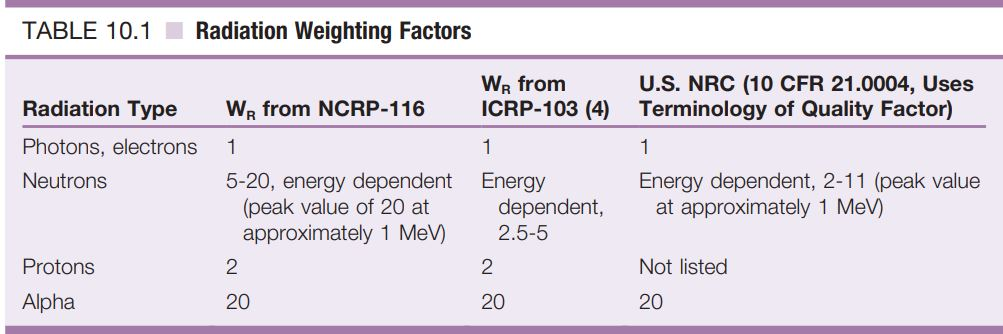
\includegraphics[width=0.8\textwidth]{Imagens/prFatorPesoRadiacao.JPG}
			}%
			\caption{Fatores de Ponderação de Radiação.}
			\label{fig:prFatorPesoRadiacao}
		\end{figure}
	
	Os fatores de ponderação da radiação são valores específicos atribuídos a diferentes tipos de radiação para levar em consideração seus efeitos biológicos relativos. Esses fatores são determinados com base em estudos epidemiológicos e estudos de radiobiologia.

	A unidade de medida padrão para a dose equivalente é o Sievert (Sv) joule por 
	quilograma (J/kg), no sistema internacional (SI). No entanto, uma unidade mais antiga, o roentgen equivalente (rem), que é igual a 0.01 Sv, também é utilizada em alguns contextos.
	
	O conceito de dose efetiva (E) leva em consideração a sensibilidade individual de cada órgão à radiação. A dose efetiva é calculada somando-se as doses equivalentes ponderadas de todos os órgãos irradiados, de acordo com os fatores de ponderação específicos de cada órgão. Esse cálculo é representado pela equação:

		\begin{equation}
			E = \sum_T W_T \cdot H_T
		\end{equation}

		\begin{exemplo}[onde,]
			\begin{itemize}
				\item \textcolor{DarkTurquoise}{$\mathbf{W_T}$} é o fator de ponderação para o órgão;
				\item \textcolor{DarkTurquoise}{$\mathbf{H_T}$} é a dose equivalente no tecido ou órgão.
			\end{itemize}
		\end{exemplo}

	Os valores para o \textcolor{MediumOrchid}{$\mathbf{W_T}$} são apresentados na \ref{fig:prFatorPesoOrgao}. A soma de todos os fatores de ponderação dos órgãos é igual a 1, ou seja $\sum W_T = 1$.

	\begin{figure}[!h]
			\centering
			\fcolorbox{DarkTurquoise}{white}{%
				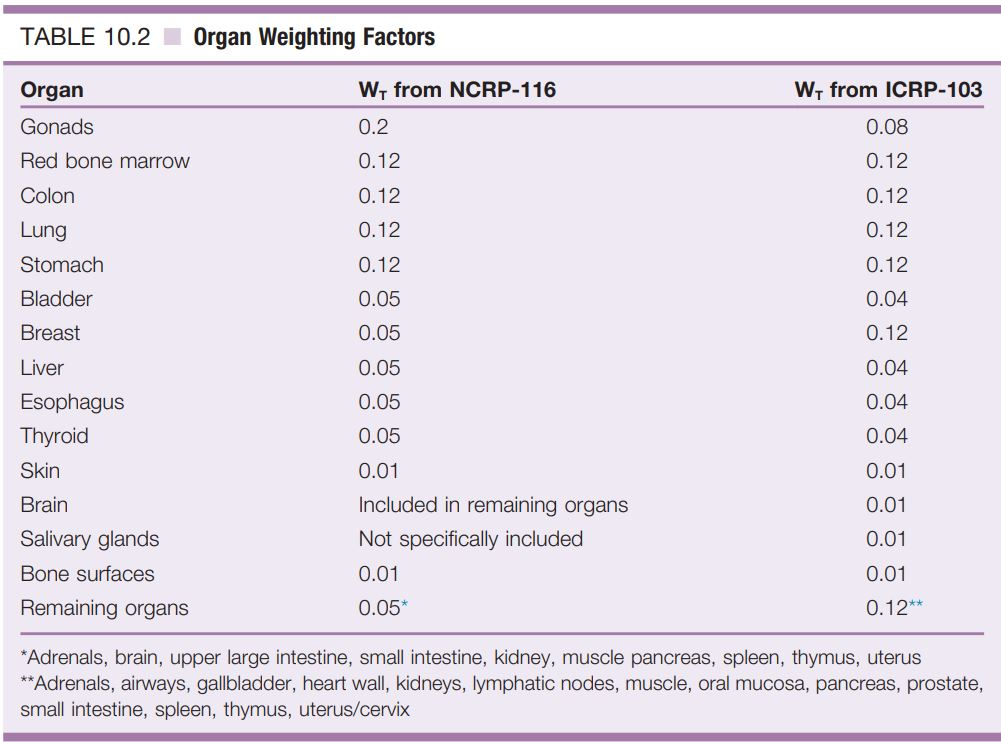
\includegraphics[width=0.8\textwidth]{Imagens/prFatorPesoOrgao.JPG}
			}%
			\caption{Fatores de Peso dos Órgãos.}
			\label{fig:prFatorPesoOrgao}
	\end{figure}

	É importante ressaltar que há debates em relação ao conceito de dose efetiva. Alguns autores argumentam que esse conceito pode ter limitações, pois envolve julgamentos subjetivos e não leva em consideração certas dependências, como a idade e o gênero do indivíduo. No entanto, a dose efetiva ainda é amplamente utilizada na radioproteção para avaliar o risco radiológico em diferentes órgãos e tecidos.


\section{Limites Regulatórios}

	O NCRP Report No. 116, publicado em 1993, é um importante documento que estabelece os limites de dose efetiva para trabalhadores expostos à radiação e o público em geral. Ele substitui o NCRP Report No. 91, lançado anteriormente em 1987. A atualização do relatório reflete o avanço do conhecimento científico e as mudanças nas diretrizes de proteção radiológica ao longo do tempo.(\ref{fig:prLimitesAnuais}).  Inicialmente, o NCRP recomendou um limite anual de dose efetiva de 0,25 mSv para o público em geral. No entanto, uma clarificação posterior em 2004 justificou o aumento desse limite para 1,0 mSv por ano. Essa alteração foi baseada em estimativas conservadoras incorporadas na metodologia de projeto de blindagem, que considera uma série de fatores para garantir a segurança radiológica.

	\begin{figure}[!h]
			\centering
			\fcolorbox{DarkTurquoise}{white}{%
				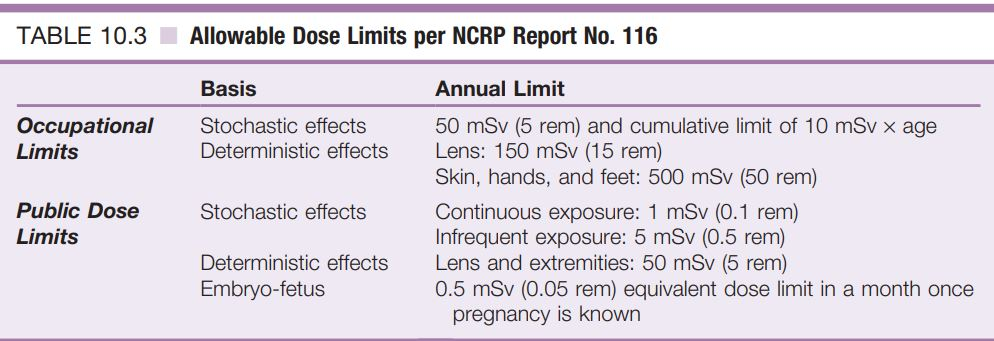
\includegraphics[width=0.8\textwidth]{Imagens/prLimitesAnuais.JPG}
			}%
			\caption{Limites de Dose Permitidos pelo Relatório NCRP nº 116.}
			\label{fig:prLimitesAnuais}
	\end{figure}

	O relatório NCRP-116 destaca a necessidade de ação corretiva quando a exposição pública a fontes naturais de radiação excede 5 mSv. Isso indica que, acima desse nível, medidas devem ser tomadas para reduzir a exposição e minimizar os riscos associados à radiação. O relatório NCRP-116 também afirma que a exposição a doses efetivas abaixo de 0.01 mSv é considerada de risco negligenciável. Isso significa que os efeitos adversos à saúde são insignificantes ou desprezíveis nesses níveis de exposição.

	Para compreender melhor esses limites, é relevante considerar a radiação de fundo natural. A radiação de fundo natural é a radiação presente no ambiente de forma natural, proveniente de várias fontes, como a radiação cósmica, a radiação proveniente do solo e materiais de construção, e a radiação proveniente de elementos radioativos presentes no corpo humano. A média da radiação de fundo natural é de aproximadamente 3.1 mSv por ano. No entanto, esse valor pode variar dependendo de fatores como a localização geográfica, a altitude e as concentrações de radônio.

	Além da radiação de fundo natural, as pessoas também são expostas à radiação por meio de procedimentos médicos. Nos Estados Unidos, em média, uma pessoa é exposta a cerca de 3 mSv por ano devido a usos médicos de radiação. A tomografia computadorizada (TC) é a principal fonte de exposição, mas também há contribuições de procedimentos realizados em medicina nuclear e radiologia intervencionista.


\section{Liberação de Pacientes com Materiais Radioativos}

	No contexto da administração ou implantação de material radioativo em pacientes, existem limites para os níveis de exposição nos quais esses pacientes podem ser liberados. O documento NUREG-1556 da U.S. NRC descreve três métodos para calcular os critérios de liberação do paciente.

	Dois Critérios de liberação são baseados na atividade administrada e na taxa de dose (\ref{fig:prCriterio}). De acordo com o NUREG-1556, se a atividade administrada for menor do que a atividade listada na coluna 1 da Tabela U1, ou se a taxa de dose medida a 1 metro for menor do que o valor listado na coluna 2 da Tabela U1, o paciente pode ser liberado. É importante observar que esses critérios não se aplicam a bebês ou crianças que são amamentados pelo paciente, para os quais instruções especiais devem ser fornecidas.  Essas instruções devem especificar a interrupção ou suspensão da amamentação e as consequências caso os níveis excedam aqueles listados na Tabela U3 (\ref{fig:prCrprAtividadesMedNuciterio}). Essas orientações se aplicam a radionuclídeos injetados usados na medicina nuclear e não são relevantes na Radioterapia.


		\begin{figure}[!h]
			\centering
			\fcolorbox{DarkTurquoise}{white}{%
				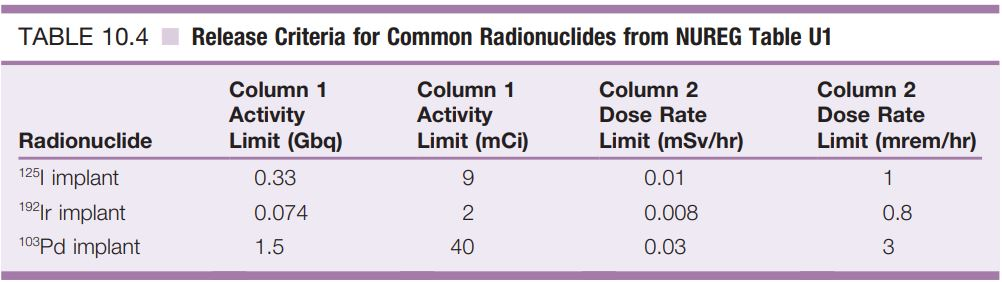
\includegraphics[width=0.8\textwidth]{Imagens/prCriterio.JPG}
			}%
			\caption{Critérios de Liberação para Radionuclídeos Comuns da Tabela U1 do NUREG.}
			\label{fig:prCriterio}
		\end{figure}


		\begin{figure}[!h]
			\centering
			\fcolorbox{DarkTurquoise}{white}{%
				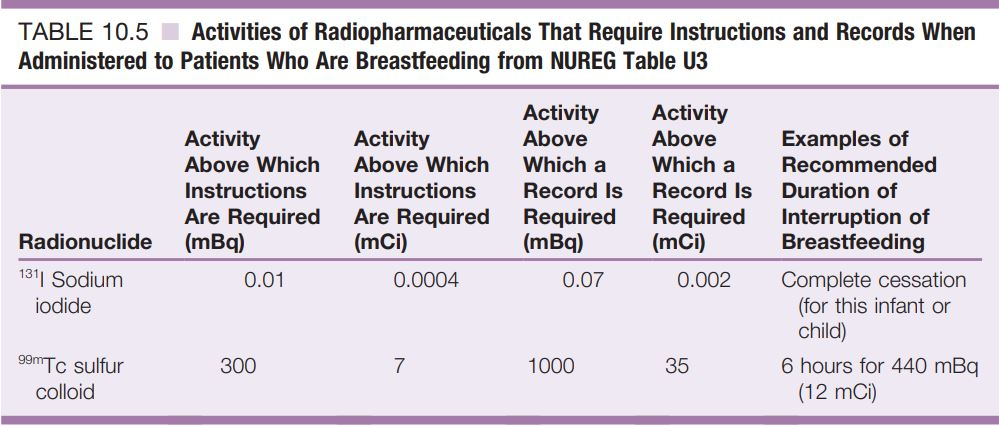
\includegraphics[width=0.8\textwidth]{Imagens/prAtividadesMedNuc.JPG}
			}%
			\caption{Atividades de radiofármacos que requerem instruções e registros quando administrados a pacientes que estão amamentando do NUREG Tabela U3.}
			\label{fig:prCrprAtividadesMedNuciterio}
		\end{figure}

	O terceiro método descrito no NUREG-1556 envolve a realização de cálculos específicos para cada paciente, garantindo que nenhum indivíduo receba uma dose efetiva superior a 5 mSv (0,5 rem). Esses cálculos podem levar em consideração fatores como meia-vida efetiva, atividade retida, fatores de ocupação inferiores a 0.25 e blindagem pelos tecidos. É importante manter um registro desses cálculos. (Esse método é importante para braquiterapia \ref{fig:prAtidadeBraq})

	\begin{figure}[!h]
		\centering
		\fcolorbox{DarkTurquoise}{white}{%
			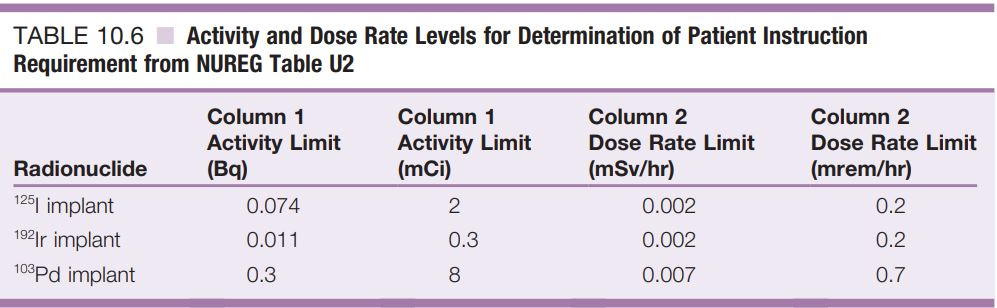
\includegraphics[width=0.8\textwidth]{Imagens/prAtidadeBraq.JPG}
		}%
		\caption{Níveis de taxa de atividade e dose para determinação do requisito de instrução do paciente da tabela NUREG U2.}
		\label{fig:prAtidadeBraq}
	\end{figure}

	É uma prática recomendada fornecer aos pacientes documentação da atividade administrada, para que eles possam esclarecer qualquer dúvida ou abordar situações como a ativação de alarmes de radiação em locais públicos. Um cartão de identificação na carteira é uma forma conveniente de fornecer essa documentação. Além disso, se as atividades ou taxa de dose a 1 metro excederem os níveis estabelecidos na Tabela U2 do NUREG-1556, instruções específicas devem ser fornecidas aos pacientes para garantir que os limites de dose aceitáveis para outras pessoas sejam mantidos.

\section{Monitoramento de Pessoal}

	O Relatório NCRP No. 102, intitulado "Proteção contra Raios X Médicos, Feixe de Elétrons e Raios Gama", enfatiza a importância da monitoração pessoal como um meio valioso para verificar a eficácia de um programa de proteção radiológica. Essa monitoração pode identificar práticas inadequadas ou incorretas de proteção radiológica, bem como situações de exposição à radiação potencialmente graves. Um resumo das recomendações do programa contidas nesse documento são:

	\begin{enumerate}
		\item Consulta a um especialista qualificado: O NCRP No. 102 destaca a importância de buscar orientação de um especialista qualificado ao estabelecer ou avaliar um programa de monitoração pessoal. Um especialista com conhecimento e experiência em proteção radiológica poderá fornecer as diretrizes adequadas e garantir que o programa esteja em conformidade com as regulamentações e práticas recomendadas.

		\item Monitoração pessoal para indivíduos ocupacionalmente expostos: O relatório recomenda que a monitoração pessoal seja realizada em indivíduos expostos ocupacionalmente que tenham uma razoável possibilidade de exceder 10\% dos limites de dose aplicáveis. Essa monitoração permite avaliar e registrar as doses de radiação recebidas pelos trabalhadores, garantindo que elas estejam dentro de limites aceitáveis.
		
		\item Investigação de casos de doses excedentes: O relatório estabelece que todos os casos relatados em que as doses excedam os limites ocupacionais devem ser investigados pelo oficial de segurança radiológica. Essa investigação é necessária para identificar as causas das doses excedentes e tomar as medidas corretivas apropriadas para prevenir exposições futuras.
		
		\item Uso dos dispositivos de monitoração: É destacado que os dispositivos utilizados para monitorar a exposição ocupacional não devem ser usados quando o indivíduo estiver exposto à radiação como paciente. Isso é importante para garantir que as doses registradas nos dosímetros reflitam exclusivamente a exposição ocupacional e não a exposição como paciente.
		
		\item Posicionamento e visibilidade dos dosímetros: O relatório recomenda que os dosímetros sejam usados de forma que sejam visíveis o tempo todo, exceto quando deliberadamente cobertos por um protetor. Isso garante que a exposição à radiação seja monitorada de maneira adequada e contínua.
		
		\item Posicionamento dos dosímetros em Radioterapia: No campo da Radioterapia, o dosímetro deve ser usado no tronco do corpo acima da cintura. Dosímetros para extremidades devem ser usados ao manipular material radioativo. Essas práticas garantem uma avaliação precisa das doses recebidas pelos profissionais de Radioterapia e auxiliam na proteção radiológica adequada durante esses procedimentos.
		
		\item Monitoração de pessoal grávido: O relatório destaca a importância de considerar a monitoração de pessoal grávido. As mulheres grávidas estão sujeitas a diretrizes específicas de proteção radiológica, levando em consideração os possíveis riscos para o feto. A monitoração pessoal adequada e a implementação de medidas de proteção adicionais são essenciais nesses casos.
	\end{enumerate}



\section{Blindagem}

	A blindagem adequada ao redor de fontes de radiação, como aceleradores lineares de MV usados em radioterapia, é crucial para garantir a segurança dos profissionais de radioterapia e do público em geral. O NCRP-151 é uma referência importante para orientar os cálculos de blindagem nesses casos. Segundo o NCRP, esses cálculos devem ser realizados por um especialista qualificado (QE), que é definido como alguém certificado pelo American Board of Radiology, American Board of Medical Physics, American Board of Health Physics ou Canadian College of Physicists in Medicine.

	Vários fatores são levados em consideração ao determinar a natureza da blindagem necessária. Esses fatores incluem:

	\begin{enumerate}
		\item Carga de trabalho (W): Refere-se à frequência com que a fonte de radiação é utilizada, levando em conta o número de pacientes sendo tratados ou examinados por semana e os tempos de tratamento ou exame.
		\item Fator de uso (U): É determinado pelas capacidades do equipamento e pelos tipos de tratamentos ou exames sendo realizados, considerando com que frequência o feixe de radiação é direcionado para uma direção específica.
		\item Barreira primária versus barreira secundária: É levado em conta se o feixe primário atinge diretamente a barreira de proteção ou não. A barreira primária é a primeira linha de defesa contra a radiação primária, enquanto a barreira secundária é exposta à radiação espalhada pelo paciente, pelos dispositivos de suporte do paciente e pelas estruturas do ambiente, ou à radiação de fuga da fonte de radiação.
		\item Fator de ocupação (T): Considera com que frequência a área adjacente à fonte de radiação é ocupada e quem a ocupa (profissional de radioterapia, área controlada ou público em geral). Isso determina o objetivo de projeto (P), que geralmente é expresso em dose efetiva por semana.
		\item Distância (d): Refere-se à distância da área de interesse em relação à fonte de radiação.
		\item Tipo de fonte de radiação: Pode variar, incluindo raios-X kV, raios-X MV, radioisótopos ou feixe de partículas.
	\end{enumerate}

	A equação básica utilizada para calcular o fator de transmissão da barreira (B) necessário para reduzir a dose efetiva em uma área para o objetivo de projeto é:
	
	\begin{equation}
		B = \frac{P \cdot d^2}{W \cdot U \cdot T}
	\end{equation}
	
	Essa equação leva em conta todos os fatores mencionados anteriormente.

	A partir do fator de transmissão (B), é possível calcular o número de camadas deci-redutoras (TVL) necessárias para reduzir a transmissão por um fator de 10. Essas camadas subsequentes, designadas como TVLe, têm valores diferentes devido a mudanças espectrais no feixe à medida que ele penetra na barreira.

	As barreiras secundárias são expostas principalmente à radiação espalhada pelo paciente. A energia e a intensidade dessa radiação espalhada dependem do ângulo em relação ao feixe primário. O feixe primário terá uma intensidade e energia muito maiores do que a radiação espalhada. A radiação de fuga, por sua vez, terá uma energia mais alta do que o feixe primário, devido ao endurecimento à medida que a radiação passa pela blindagem da fonte, mas terá uma intensidade muito menor. Normas como a IEC 60601-2-1 limitam a radiação de fuga ao redor do cabeçote de um acelerador linear a menos de 0.1\% do feixe primário a 1 metro de distância do cabeçote.

	Os fatores de ocupação (T) são projetados para reduzir a necessidade de blindagem em áreas com baixa probabilidade de ocupação humana. No entanto, ao realizar cálculos de blindagem para uma área de baixa ocupação, como um banheiro público, a dose também deve ser avaliada para áreas de alta ocupação adjacentes, como um escritório completamente ocupado. Isso determinará a blindagem necessária nessa direção específica. Os fatores de ocupação recomendados pelo NCRP-151 estão mostrados na \ref{fig:prFatorOcupacao}.

	\begin{figure}[!h]
		\centering
		\fcolorbox{DarkTurquoise}{white}{%
			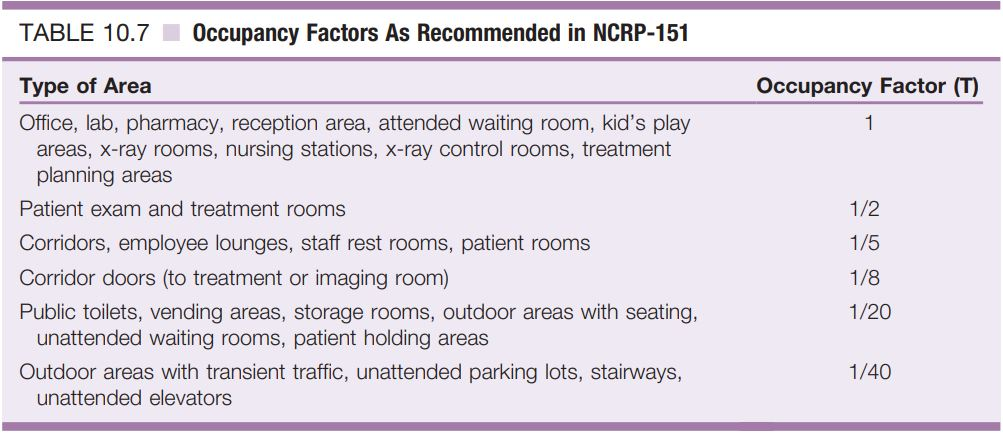
\includegraphics[width=0.8\textwidth]{Imagens/prFatorOcupacao.JPG}
		}%
		\caption{Fatores de ocupação conforme recomendado em NCRP-151.}
		\label{fig:prFatorOcupacao}
	\end{figure}

	É importante observar que nenhuma barreira pode eliminar completamente a dose de radiação ao redor de uma fonte de radiação, mas é essencial reduzi-la a níveis seguros. O princípio ALARA (As Low As Reasonably Achievable - Tão Baixo Quanto Razoavelmente Atingível) é relevante aqui, enfatizando a necessidade de minimizar a exposição à radiação sempre que possível. 
	
	O NCRP recomenda o uso de um objetivo de projeto (P) de 0.1 mSv/semana (10 mrem) para áreas controladas e 0.02 mSv/semana (2 mrem) para áreas livres. Esses valores correspondem a níveis de dose aproximadamente 10 vezes menores do que a dose máxima permitida para um trabalhador ocupacional.

	Além dos cálculos mencionados acima, é essencial manter a taxa de dose em uma área pública abaixo de um certo limite, independentemente do fator de ocupação. Isso é necessário para evitar a exposição de indivíduos que estejam ocupando o espaço quando o feixe de radiação for direcionado a eles. Nessa situação, a dose efetiva poderia exceder o limite semanal em um curto período de tempo. Os limites relevantes são de 0.02 mSv (2 mR) em qualquer uma hora. Às vezes, essa restrição acaba sendo o principal fator determinante em um cálculo de blindagem.

\subsection*{BLindagem MV}


	O \textit{NCRP-151}, intitulado \textit{Projeto e Avaliação de Blindagem Estrutural para Instalações de Radioterapia com Raios-X e Gama de Megavoltagem}, é um recurso fundamental para a determinação da blindagem necessária em radioterapia de megavoltagem (MV). A Agência Internacional de Energia Atômica (IAEA) também emitiu um relatório chamado "Proteção Radiológica no Projeto de Instalações de Radioterapia". Ao projetar barreiras de blindagem para aceleradores lineares de MV, é essencial considerar quatro fontes principais de radiação:

		\begin{enumerate}
		\item Feixe primário ($B_{\text{pri}}$)
		\item Espalhamento pelo paciente ($B_{\text{ps}}$)
		\item Fuga no cabeçote ($B_{\text{L}}$)
		\item Nêutrons (se > \SI{10}{\mega\volt})
		\end{enumerate}

	Existem equações relevantes para calcular os componentes de fótons:

		\begin{equation}
		B_{\text{pri}} = \frac{P \cdot d_{\text{pri}}^2}{{W \cdot U \cdot T}}
		\end{equation}

		\begin{equation}
		B_{\text{ps}} = \frac{{P \cdot d_{\text{sca}}^2 \cdot d_{\text{sec}}^2 \cdot 400}}{{\alpha \cdot W \cdot T \cdot F}}
		\end{equation}

		\begin{equation}
		B_{\text{L}} = \frac{{P \cdot d_{\text{L}}^2}}{{10^{-3} \cdot W \cdot T}}
		\end{equation}

		\begin{exemplo}[Onde:]
			\begin{itemize}
			\item $d_{\text{pri}}$, $d_{\text{sca}}$, $d_{\text{sec}}$ e $d_{\text{L}}$ são distâncias descritas na Figura \ang{10.1}. Essas distâncias são medidas a \SI{30}{\centi\meter} da superfície externa da parede ou porta para representar um espaço ocupável.
			\item $\alpha$ = fração de espalhamento para um determinado ângulo
			\item $F$ = área do campo na meia profundidade do paciente a \SI{1}{\meter}
			\end{itemize}
		\end{exemplo}

		\begin{figure}[!h]
			\centering
			\fcolorbox{DarkTurquoise}{white}{%
				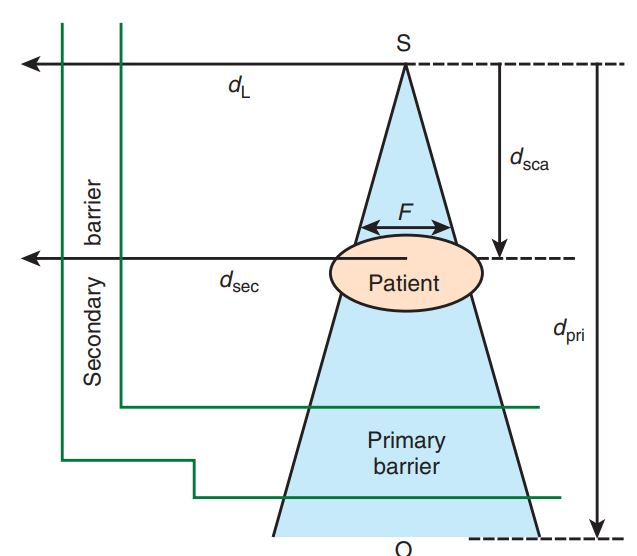
\includegraphics[width=0.5\textwidth]{Imagens/prLayoutSala.JPG}
			}%
			\caption{Layout da sala mostrando as distâncias associadas à radiação espalhada e de fuga.}
			\label{fig:prLayoutSala}
		\end{figure}

	O fator $10^{-3}$ em $B_{\text{L}}$ é utilizado para considerar que a fuga de radiação no cabeçote é menor que 0.1\% do feixe primário a \SI{1}{\meter}.

	Para $d_{\text{sca}} = \SI{1}{\meter}$, que é um valor típico, e um campo de $20 \times 20 = \SI{400}{\centi\meter\squared}$ (cancelando o fator de 400), a equação para $$B_{\text{ps}}$$ se torna $$B_{\text{ps}} = \frac{{P \cdot d_{\text{sec}}^2}}{{\alpha \cdot W \cdot T \cdot F}}$$ Portanto, se $\alpha$ for muito menor que o fator $10^{-3}$ na fórmula para fuga, a radiação de fuga terá maior influência no cálculo da barreira secundária. As frações de espalhamento mostradas na \ref{fig:prFracaoEspalhamento} confirmam que isso é verdadeiro em muitos casos.

	\begin{figure}[!h]
		\centering
		\fcolorbox{DarkTurquoise}{white}{%
			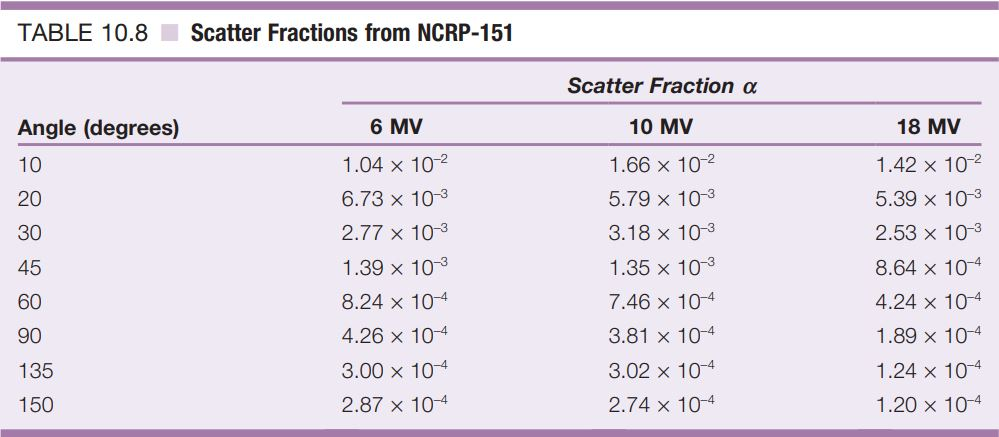
\includegraphics[width=0.8\textwidth]{Imagens/prFracaoEspalhamento.JPG}
		}%
		\caption{Frações de dispersão de NCRP-151.}
		\label{fig:prFracaoEspalhamento}
	\end{figure}

	Reorganizando qualquer uma dessas equações, é possível calcular a dose equivalente ($H$). Por exemplo:

		\begin{equation}
		H_{\text{pri}} = \frac{{W \cdot U \cdot T \cdot B_{\text{pri}}}}{{d^2}}
		\end{equation}

	onde $H_{\text{pri}}$ é medido em microsieverts ($\mu$Sv) por semana.

	É importante observar que a carga de trabalho, $W$, para $B_{\text{pri}}$ e $B_{\text{ps}}$ é baseada na dose semanal no isocentro, enquanto $W$ para $B_{\text{L}}$ é baseada no tempo total de irradiação. No caso de técnicas como IMRT ou terapia de arco modulado volumétrico (VMAT), em que mais unidades monitoras (MU) são entregues por unidade de dose (e os tempos totais de irradiação são mais longos), o valor de $B_{\text{L}}$ na equação de fuga deve ser ajustado considerando essa diferença. Esse ajuste é conhecido como "fator IMRT", representado por $CI$, que é igual a $$CI = \frac{{MU_{\text{IMRT}}}}{{MU_{\text{convencional}}}}$$ Valores típicos para $CI$ variam de 3 a 5, mas podem ser maiores (10 a 15) em casos especiais, como TomoTherapy e CyberKnife.

	O fator de uso da barreira primária ($U$) para um acelerador linear moderno é detalhado no \textit{NCRP-151} e é mostrado na \ref{fig:prFatorUso}. Os valores são fornecidos dependendo se são utilizados os 4 ângulos cardinais para cálculo ou uma faixa variação de \ang{45}. Essa abordagem difere da metodologia histórica, que considerava 0.25 para cada um dos ângulos cardinais (0, 90, 180, 270). 

	\begin{figure}[!h]
		\centering
		\fcolorbox{DarkTurquoise}{white}{%
			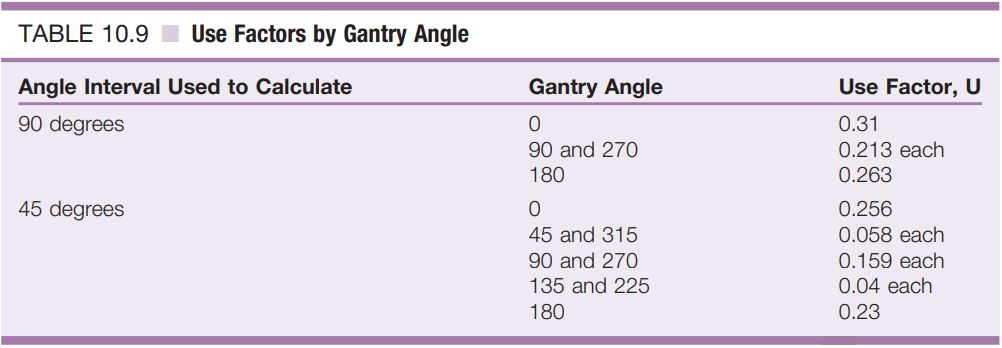
\includegraphics[width=0.8\textwidth]{Imagens/prFatorUso.JPG}
		}%
		\caption{Fator de Uso por ângulo do gantry.}
		\label{fig:prFatorUso}
	\end{figure}
	
	A largura da barreira primária deve ser a largura do tamanho máximo do campo projetado na distância da barreira mais \SI{30}{\centi\meter} em cada lado. A largura do tamanho máximo do campo geralmente é a diagonal do tamanho máximo do campo. A distância usada para calcular a projeção do tamanho máximo do campo varia com base se a barreira se estende para dentro da sala (\ref{fig:prPrim}). Usando essa relação, a barreira geralmente também abrangerá a área de \ang{20} de espalhamento que contém a contribuição máxima de espalhamento. Se a quantidade de espaço ocupado pela barreira primária precisar ser reduzida, é possível utilizar uma combinação de concreto, chumbo ou aço. No caso de energias superiores a \SI{10}{\mega\volt}, a quantidade de concreto deve ser suficiente para absorver os nêutrons ou igualar a espessura da barreira secundária. As camadas deci-redutoras (TVLs) da barreira primária para várias energias e materiais estão listadas na \ref{fig:prTvlPrim}.

	\begin{figure}[h]
		\centering
		\subfigure{
			\fcolorbox{DarkTurquoise}{white}{%
				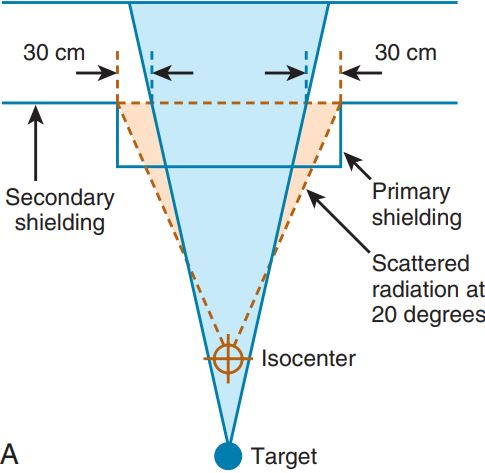
\includegraphics[width=0.3\textwidth]{Imagens/prPrim1.JPG}
			}}
		\subfigure{
			\fcolorbox{DarkTurquoise}{white}{%
				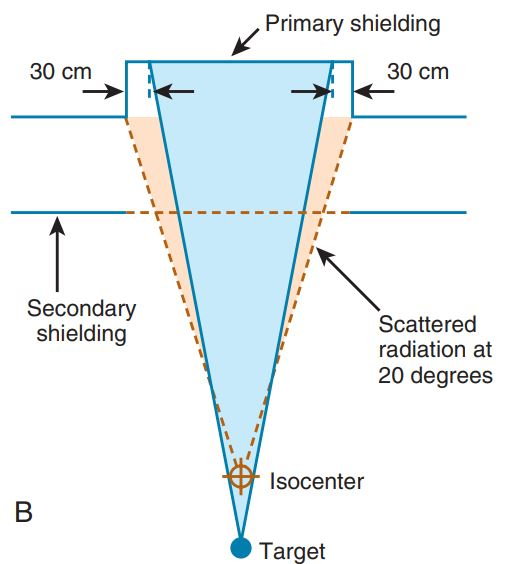
\includegraphics[width=0.3\textwidth]{Imagens/prPrim2.JPG}
			}} \\ %
		\subfigure{
			\fcolorbox{DarkTurquoise}{white}{%
				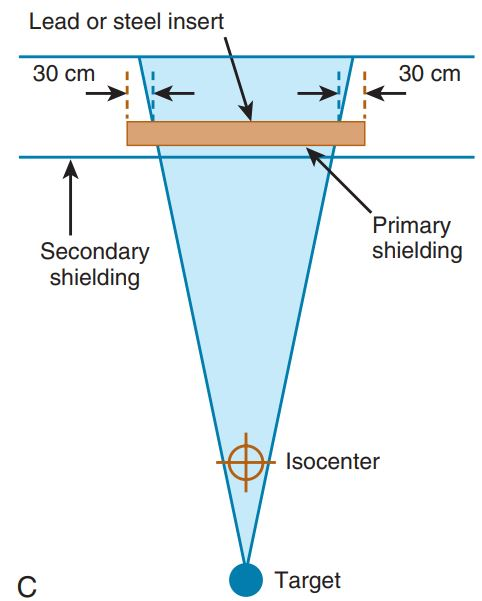
\includegraphics[width=0.3\textwidth]{Imagens/prPrim3.JPG}
		}} \\ %
		\caption{Determinação da largura da barreira primária para várias configurações de barreira.}
		\label{fig:prPrim}
	\end{figure}


	As barreiras secundárias devem levar em consideração tanto a fuga quanto o espalhamento. Na prática, a barreira secundária é calculada independentemente para o fuga e o espalhamento. Se os dois valores estiverem dentro de uma diferença de camada semi-redutora (HVL), então uma HVL deve ser adicionada à maior delas e usada como espessura da barreira. Uma HVL é equivalente a 0.33 TVL. As TVLs para fuga e espalhamento são fornecidas na \ref{fig:prTvlFul} e \ref{fig:prTvlEsp}, respectivamente.

	\begin{figure}[h]
		\centering
		\fcolorbox{DarkTurquoise}{white}{%
			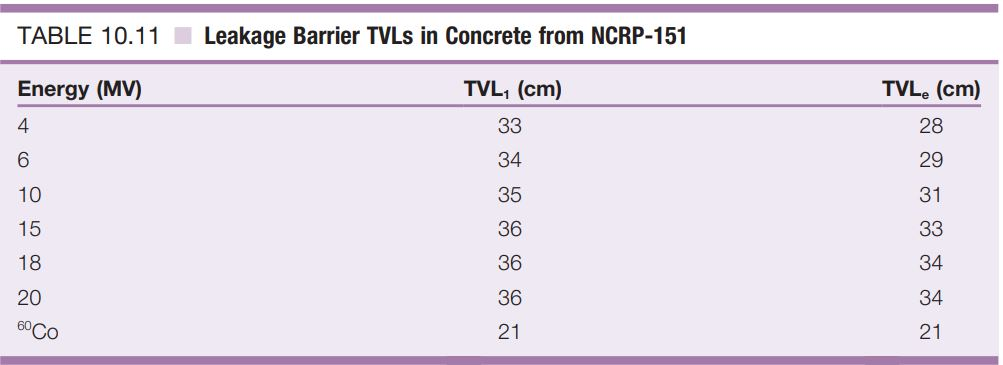
\includegraphics[width=0.8\textwidth]{Imagens/prTvlFul.JPG}
		}%
		\caption{TVL de barreira para radiação de fuga NCRP-151.}
		\label{fig:prTvlFul}
	\end{figure}

	\begin{figure}[h]
		\centering
		\fcolorbox{DarkTurquoise}{white}{%
			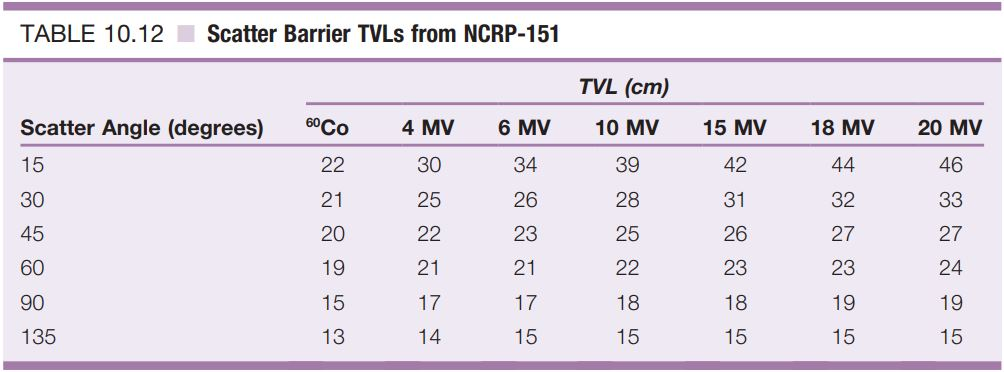
\includegraphics[width=0.8\textwidth]{Imagens/prTvlEsp.JPG}
		}%
		\caption{TVL barreira radiação espalhada NCRP-151.}
		\label{fig:prTvlEsp}
	\end{figure}

	Como mencionado anteriormente, há um limite de \SI{0.02}{\milli\sievert} em qualquer uma hora. Uma vez que os aceleradores lineares emitem feixes pulsados e os pacientes geralmente são tratados em períodos de 10 a 20 minutos, com o tempo real de irradiação sendo uma fração pequena desse tempo, a taxa de dose instantânea (IDR) pode exceder \SI{0.02}{\milli\sievert}/hora e ainda estar em conformidade com o limite de \SI{0.02}{\milli\sievert} em qualquer uma hora, desde que $W$ não seja extremamente baixo. O conceito de taxa média de dose equivalente ao longo do tempo (TADR), representada por $R_W$, ajuda a explicar isso. $RW$ é calculado pela fórmula:

	\begin{equation}
	R_W = \frac{\text{IDR} \cdot W_\text{pri} \cdot U_\text{pri}}{D_0}
	\end{equation}

	Onde $D_0$ é a saída a \SI{1}{\meter}. Conceptualmente, $R_W$ é sempre menor ou igual a P/horas de operação (por exemplo, uma semana de trabalho de 40 horas). Se $R_W \cdot T$ for menor que $P$, então a barreira é considerada adequada. Reorganizando a fórmula, temos o seguinte resultado:

	\begin{equation}
	\text{IDR} <  \frac{P \cdot D_0}{W \cdot U \cdot T} 
	\end{equation}

	\begin{tcolorbox}[width=\textwidth, colback={white}, colbacktitle={DarkTurquoise!50!white}, title={$\bigstar$ \LobsterTwo{Exemplo: IDR} $\bigstar $}, coltitle={CarnationPink}, colframe={DarkTurquoise}, fonttitle=\rmfamily\bfseries\Large, breakable]
		Se,
		\begin{itemize}
			\item \textcolor{DarkTurquoise}{$\mathbf{P}$}$= \SI{0.02}{\milli\sievert}/\text{semana}$
			\item \textcolor{DarkTurquoise}{$\mathbf{D_0}$}$= \SI{4}{\gray}/\text{min}$
			\item \textcolor{DarkTurquoise}{$\mathbf{W}$}$= \SI{750}{\gray}/\text{semana}$ e
			\item \textcolor{DarkTurquoise}{$\mathbf{U}$}$= 0.213$
		\end{itemize}

		 Então a IDR deve ser menor que \textcolor{MediumOrchid}{\textbf{\SI{0.0005}{\milli\sievert}/\text{min}}} ou \textcolor{MediumOrchid}{\textbf{\SI{0.03}{\milli\sievert}/\text{hora}}}.
		 
		 \

		 Na prática, as agências reguladoras podem limitar a IDR máxima, mesmo se o limite de \SI{0.02}{\milli\sievert} em qualquer uma hora for cumprido. No Reino Unido, por exemplo, há um limite de \SI{7.5}{\micro\sievert}/hora em áreas não controladas.
	\end{tcolorbox}

	Considerações especiais devem ser feitas para penetrações na parede, como conduítes e dutos de ar. Quando possível, as penetrações na parede devem ser anguladas para que não haja um caminho direto através delas. É aconselhável ter uma curva na penetração. Isso pode não ser possível para dutos de ar grandes, que exigirão defletores de blindagem (consulte a Figura \ref{fig:prductos}). Além disso, procedimentos especiais, como a irradiação corporal total (TBI), precisarão ser abordados de forma específica. Devido aos longos tempos de irradiação envolvidos, a IDR pode precisar ser ainda mais baixa nesses casos.

	\begin{figure}[!h]
		\centering
		\fcolorbox{DarkTurquoise}{white}{%
			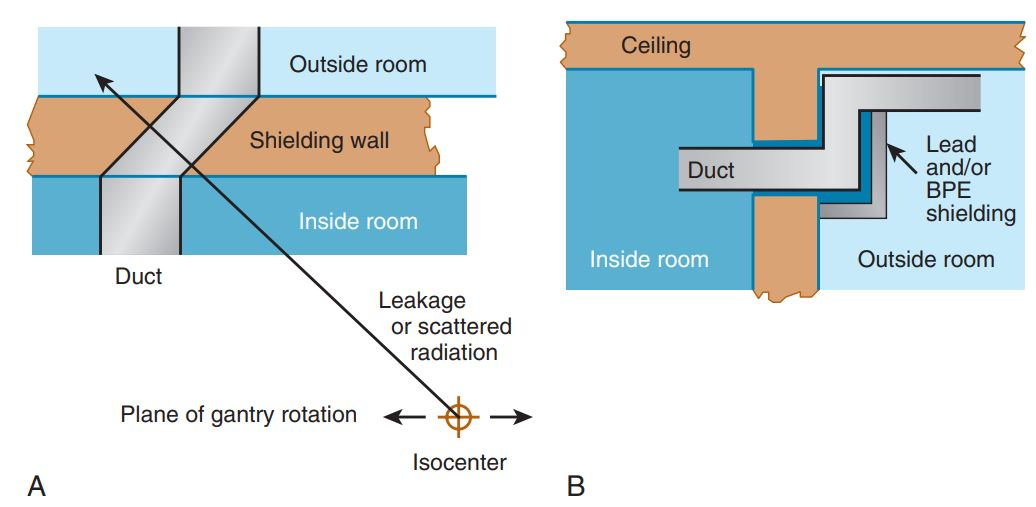
\includegraphics[width=0.8\textwidth]{Imagens/prductos.JPG}
		}%
		\caption{Métodos de penetração em dutos.}
		\label{fig:prductos}
	\end{figure}

	Se não houver ocupação acima da sala, a blindagem do teto pode ser relativamente fina. Nesse caso, os requisitos de espessura da blindagem podem ser determinados pelo espalhamento pelo teto e pelo retorno na outra face da parede ou para uma área ou prédio adjacente. Isso é conhecido como "skyshine". O \textit{NCRP-151} fornece a seguinte equação para calcular a taxa de dose equivalente do skyshine ($H$):

	\begin{equation}
		H = \frac{2.5 \times 10^7  \cdot ( B_{\text{XS}} D_0 \cdot \Omega)^{1.3}}{(dI \cdot dS)^2 }
	\end{equation}

	Onde:
	\begin{itemize}
	\item $(2.5 \times 10^7)$ converte \si{\gray} para \si{\nano\sievert}
	\item $B_{\text{XS}}$ = fator de transmissão da blindagem do teto para fótons
	\item $D_0$ = saída a \SI{1}{\meter} (\si{\gray}/\si{\hour})
	\item $\Omega$ = ângulo sólido do feixe máximo (esterradianos)
	\item $dI$ = distância do alvo a um ponto \SI{2}{\meter} acima do teto
	\item $dS$ = distância do isocentro até o ponto de cálculo no outro lado da parede
	\end{itemize}

	O skyshine é especialmente importante em salas de tratamento onde não há espaço ocupado acima. Se esse espaço for um teto com acesso para manutenção, pode ser necessário considerá-lo como uma área pública e/ou controlada de alguma forma. Um fenômeno semelhante pode ocorrer através do piso, conhecido como "groundshine".

	A blindagem para nêutrons é, de certa forma, mais simples e, de outras formas, mais complicada. Materiais com alta concentração de hidrogênio são particularmente eficazes na blindagem de nêutrons térmicos devido à sua alta seção transversal de absorção de nêutrons. Para as paredes principais do bunker, se houver concreto suficiente para blindar o espalhamento e a fuga de alta energia (> \SI{10}{\mega\volt}), haverá também blindagem suficiente para os nêutrons. O concreto possui um alto teor de água e hidrogênio, o que o torna um bom absorvedor de nêutrons. O chumbo é principalmente transparente para nêutrons. Se o chumbo for usado como material de blindagem primária em um bunker de alta energia, ele precisará ser confinado com concreto ou aço devido à falta de integridade estrutural. Se o aço for usado como suporte ou se não houver concreto suficiente para blindar o espalhamento e a fuga de fótons, pode-se utilizar um material de blindagem de nêutrons, como o polietileno. O polietileno pode ser dopado com boro para aumentar a eficiência da blindagem contra nêutrons.

	O aspecto mais complexo da blindagem em uma sala de megavoltagem é o labirinto e a porta. Três componentes são considerados:

		\begin{enumerate}
		\item Espalhamento e fuga de fótons ($H_{\text{Tot}}$)
		\item Produção de raios gamas de captura de nêutrons ($H_{\text{cg}}$)
		\item Nêutrons ($H_{\text{n}}$)
		\end{enumerate}

	As equações são bastante complexas, sendo recomendável consultar o \textit{NCRP-151} diretamente para obter os detalhes. Em geral, fatores como o número de trajetórias de espalhamento necessárias para alcançar a porta, a área de seção transversal da entrada do labirinto para o corredor do labirinto e o uso de materiais absorvedores no final do labirinto (como polietileno borado) contribuem para o cálculo da blindagem. Se a blindagem contra nêutrons for necessária para uma porta, geralmente é recomendado o uso de polietileno borado no lado interno da porta, com chumbo ou aço no lado externo para blindar os fótons produzidos pelas interações de nêutrons térmicos no plástico.

	Considerações especiais devem ser feitas para unidades como TomoTherapy e CyberKnife. Além do aumento das unidades monitoras (MU) mencionado anteriormente, as características do feixe primário são diferentes. O TomoTherapy possui um beam stopper que atenua uma parte significativa do feixe primário. O \textit{NCRP-151} cita um valor de atenuação de $4.1 \times 10^{-3}$ medido pelo fornecedor. O braço robótico do sistema CyberKnife permite uma distribuição quase isotrópica das direções do feixe, o que torna cada parede, piso e teto uma barreira primária. As distâncias do isocentro para ambas as unidades são não padronizadas, sendo \SI{85}{\centi\meter} para o TomoTherapy e \SI{90}{\centi\meter} a \SI{100}{\centi\meter} para o CyberKnife. O \textit{NCRP} discute essas duas unidades, além de outras referências. Além disso, os planning guides, fornecidos pelo fornecedor (\textit{Accuray}), para essas unidades contêm informações úteis sobre a blindagem necessária.

	\begin{tcolorbox}[width=\textwidth, colback={white}, colbacktitle={DarkTurquoise!50!white},title={$\bigstar$ \LobsterTwo{Cálculo de Blindagem MV} $\bigstar $}, coltitle={CarnationPink}, colframe={DarkTurquoise}, fonttitle=\rmfamily\bfseries\Large, breakable]

		\begin{itemize}[label=\textcolor{CarnationPink}{$\star$}]
			\item Consideraremos uma carga de trabalho de 40 pacientes por dia em um acelerador linear de dupla energia, com feixes de 6 e 18 MV, distribuídos igualmente entre as energias. Isso resulta em uma carga de trabalho (\(W\)) de \SI{300}{\gray}/semana no isocentro para cada energia, calculada como \(20\) pacientes/dia \(\times\) \(5\) dias/semana \(\times\) \SI{3}{\gray}/paciente.
			\item No caso de uma barreira primária, assumiremos uma área livre totalmente ocupada (\(T = 1\)), com uma taxa de dose de referência (\(P\)) de \SI{0.02}{\milli\gray}/semana e um fator de utilização (\(U\)) de \ang{90}. Para uma distância de \SI{5}{\meter}, a espessura necessária seria de aproximadamente \SI{221.6}{\centi\meter} de concreto. Já para uma distância de \SI{7}{\meter}, a espessura exigida seria de \SI{209}{\centi\meter} de concreto. Dessa forma, podemos observar que a distância (de acordo com a lei do inverso do quadrado) pode ser um fator eficaz na blindagem. Além disso, salas maiores não só oferecem maior funcionalidade, como também requerem menor investimento financeiro para a implementação da blindagem necessária.
			\item Ao realizar o mesmo cálculo para o feixe de 6 MV, obtemos uma espessura necessária de \SI{172.5}{\centi\meter} de concreto a uma distância de \SI{5}{\meter}. Essa diferença de \SI{49}{\centi\meter} em relação à espessura exigida para o feixe de 18 MV representa aproximadamente 1,4 camadas de valor décimo (TVL) para o feixe de 6 MV. Consequentemente, a dose associada ao feixe de 6 MV será cerca de \(10^{-1.4}\) menor do que a dose do feixe de 18 MV, ou seja, aproximadamente 4\% da dose do feixe de 18 MV. Considerando as suposições cautelosas adotadas, como a dose de \SI{3}{\gray} por paciente, a blindagem projetada para o feixe de maior energia, com uma distribuição 50/50, também será suficiente para o feixe de menor energia.
			\item É importante considerar alguns fatores adicionais, como evitar a colocação de áreas livres totalmente ocupadas em proximidade com uma barreira primária. Optar por uma área controlada ou um corredor a uma distância de \SI{5}{\meter} reduziria a espessura necessária para aproximadamente \SI{191.5}{\centi\meter}, representando uma redução de \SI{30}{\centi\meter} em relação à espessura anteriormente mencionada.
			\item Ao realizar o cálculo para a barreira de fuga, com base nas mesmas suposições mencionadas anteriormente, obtemos uma espessura de \SI{95}{\centi\meter} para uma área não controlada totalmente ocupada a \SI{5}{\meter}. Caso haja a implementação de uma área controlada ou um corredor, a espessura necessária pode ser reduzida para \SI{72}{\centi\meter}.
		\end{itemize}
	\end{tcolorbox}
	
\subsection*{Blindagem KV}

	Na área da Radioterapia, um simulador de Tomografia Computadorizada (TC) dedicado pode exigir blindagem. Caso seja necessária, geralmente utiliza-se uma blindagem de 1.5 mm (\(\frac{1}{16}"\)) ou 0.75 mm (\(\frac{1}{32}"\)) de chumbo incorporado em gesso (drywall). O chumbo deve se estender por pelo menos 2 metros do chão, caso não haja ocupação acima da unidade. Todas as molduras de portas, maçanetas, caixas elétricas, entre outros elementos, devem ter a mesma equivalência de chumbo ou serem revestidos com chumbo. Os equipamentos de TC são auto-blindados em relação ao feixe primário, uma vez que ele é completamente interceptado pelos detectores. O espalhamento proveniente do paciente é a principal fonte de exposição. O documento NCRP-147 detalha a metodologia de blindagem.

	A equação geral para calcular a atenuação necessária (\(B\)) em uma barreira é dada por:
	\begin{equation}
	B = \frac{\kappa \times  \text{fatores para levar em conta o contraste, doses periféricas, pitch} \times  (\text{DLP})}{d^2}
	\end{equation}

	A fração de espalhamento (\(\kappa\)) a 1 m é geralmente considerada como \(9 \times 10^{-5}\) para varreduras de crânio e \(3 \times 10^{-4}\) para varreduras de corpo. Para obter a dose espalhada a 1 m (\(K^1\)), o produto de dose por comprimento (DLP) é multiplicado por \(\kappa\). Valores típicos de DLP são \SI{1200}{\milli\gray} para varreduras de cabeça e \SI{550}{\milli\gray} para varreduras de corpo, porém valores exatos devem ser obtidos junto ao fabricante. Um fator de 1.2 é aplicado à fração de espalhamento para varreduras de corpo para levar em conta o aumento da dose periférica em varreduras de corpo e o pitch em varreduras helicoidais (assumido como 1.35). O pitch para varreduras de cabeça é assumido como 1. Portanto:

	\begin{equation}
		K_{\text{head}}^1 = \SI{1200}{\milli\gray} \times 9 \times 10^{-5} = \SI{0.108}{\milli\gray}
	\end{equation}
	\begin{equation}
	K_{\text{corpo}} = 1.2 \times \SI{550}{\milli\gray} \times 3 \times 10^{-4} = \SI{0.198}{\milli\gray}
	\end{equation}

	Se forem realizadas 20 varreduras de cabeça e 40 varreduras de corpo por semana, o kerma semanal total não blindado é de \SI{10.08}{\milli\gray} a 1 m. Caso seja utilizado contraste intravenoso e sejam feitas varreduras pré e pós-contraste, o valor deve ser multiplicado por um fator de 1 mais a fração de estudos de varredura pré-/pós-contraste. Por exemplo, se 40\% das varreduras forem pré-/pós-contraste, o fator seria 1.4. O kerma total não blindado semanal à distância da área a ser blindada (\(K_0\)) é então calculado pela lei do inverso do quadrado. Portanto, se a distância (\(d\)) for de \SI{3}{\meter}, \(K_0\) para o exemplo acima é de \(\SI{10.08}{\milli\gray} \times \left(\frac{1}{3}\right)\), o que resulta em \SI{1.12}{\milli\gray}/semana.

	A atenuação necessária da barreira (\(B\)) é calculada dividindo-se a meta de projeto (\(P\)) por \(K_00\). Portanto, se a área for uma área livre, \(P = \SI{0.02}{\milli\gray}\), \(B = 0.018\) para este exemplo. As figuras A.2 e A.3 do NCRP-147 fornecem a espessura do material necessária com base na atenuação (\(B\)) para chumbo e concreto, respectivamente. Utilizando esse valor para \(B\), obtemos uma espessura de barreira de \SI{0.6}{\milli\meter} de chumbo ou \SI{65}{\milli\meter} de concreto. A espessura também pode ser encontrada ajustando os dados nas Figuras A.2 e A.3 para a Equação A.2 no relatório:
	
	\begin{equation}
		B = \left[\left(1 + \beta/\alpha\right) e^{\alpha \beta \gamma} - \beta/\alpha\right]^{-1/\gamma}
	\end{equation}

	Onde \(x\) é a espessura do material.

	Ao resolver a equação para \(x\), obtemos:

	\begin{equation}
		x = \left(\frac{1}{\alpha/\gamma}\right) \ln \left[\frac{B^{-\gamma} + \beta/\alpha}{1 + \beta/\alpha}\right]
	\end{equation}

	Os parâmetros da equação são mostrados na \ref{fig:prTransmiss} para chumbo e concreto.


		\begin{figure}[!h]
			\centering
			\fcolorbox{DarkTurquoise}{white}{%
				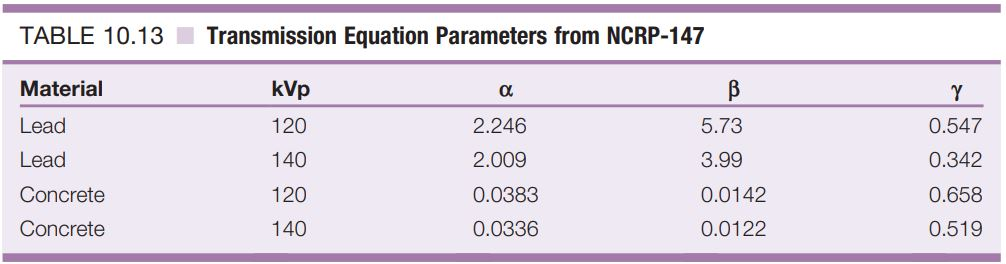
\includegraphics[width=0.8\textwidth]{Imagens/prTransmiss.JPG}
			}%
			\caption{Parâmetros de Equação de Transmissão de NCRP-147.}
			\label{fig:prTransmiss}
		\end{figure}

\subsection*{Blindagem Para Emissão de Pósitrons}

	O relatório AAPM 108 aborda os requisitos de blindagem para uma unidade de Tomografia por Emissão de Pósitrons (PET)/TC. Os fótons de aniquilação dos radionuclídeos utilizados no PET possuem uma energia de \SI{511}{\kilo\electronvolt}, o que é significativamente mais alto em comparação com outras modalidades de imagem diagnóstica. Além disso, como o próprio paciente se torna a fonte de radiação após a injeção do radionuclídeo, a movimentação do paciente pela clínica apresenta desafios adicionais.

	Durante um exame de PET, o paciente é injetado com o radionuclídeo e, em seguida, espera-se aproximadamente 60 minutos para permitir a captação do radiotraçador. Durante esse período, o paciente é colocado em uma área de repouso tranquila para reduzir a captação não específica do radiotraçador. Uma sala designada para a captação é utilizada para esse propósito e, a menos que seja excepcionalmente grande, essa sala deve ser blindada. Em seguida, o paciente é levado para a sala de imagem.

	Devido às meias-vidas muito curtas dos radionuclídeos usados no PET, o requisito de blindagem é reduzido devido ao decaimento radioativo. O fator de decaimento para um intervalo de tempo de 60 minutos para o radionuclídeo mais comum no PET, o fluorodesoxiglicose (FDG), é de 0.68. Além disso, se o paciente for orientado a urinar antes do exame, aproximadamente 15\% do radiotraçador será removido do corpo.

	A blindagem do teto e do piso deve ser cuidadosamente avaliada devido à alta energia dos fótons de aniquilação. Outras considerações para a blindagem de uma sala de PET/TC incluem a localização de outros dispositivos de imagem e instrumentos sensíveis, como contadores cintilantes e sondas de captação de tireoide. As câmeras cintilantes devem ser posicionadas de forma que os detectores nunca fiquem direcionados diretamente para uma sala de captação ou imagem. Os contadores sensíveis não devem apresentar um fundo ambiental acima de \SI{1000}{\per\minute} e devem ser localizados em áreas isoladas, longe das salas de captação e imagem. As portas das salas de imagem e captação devem ser cuidadosamente posicionadas para minimizar a quantidade de chumbo necessária, ou seja, devem ser colocadas o mais distante possível e em direção a áreas com baixa ocupação.

	As equações para calcular a atenuação necessária (B) são as seguintes:

	Para a sala de captação:
	\begin{equation}
		B = \frac{{218 \times d^2 }}{{T \times N_{\text{W}} \times A_{\text{0}} \times t_{\text{U}} \times R_{\text{tU}}}}
	\end{equation}

	Para a sala de imagem:
	\begin{equation}
		B = \frac{{256 \times d^2 }}{{T \times N_{\text{W}} \times A_{\text{0}} \times F_{\text{U}} \times t_{\text{I}} \times R_{\text{tI}}}}
	\end{equation}

	\begin{exemplo}[onde]
		\begin{itemize}
			\item \textcolor{DarkTurquoise}{$\mathbf{T}$} = \text{fator de ocupação} 
			\item \textcolor{DarkTurquoise}{$\mathbf{N}$} = \text{número de pacientes por semana} 
			\item \textcolor{DarkTurquoise}{$\mathbf{A_{\text{0}}}$} = \text{atividade administrada (MBq)} 
			\item \textcolor{DarkTurquoise}{$\mathbf{t_{\text{U}}}$} = \text{tempo de captação (horas)}
			\item \textcolor{DarkTurquoise}{$\mathbf{R_{\text{tU}} \text{ e } R_{\text{tI}}}$} = \text{fator de redução de dose ao longo do tempo de captação ou imagem}
			\item \textcolor{DarkTurquoise}{$\mathbf{F_{\text{U}}}$} = \text{fator de decaimento de captação}
		\end{itemize}
		
	\end{exemplo}

	Os fatores 0.218 e 0.256 são derivados do pressuposto de que a taxa de dose do paciente imediatamente após a injeção é de \SI{0.092}{\mu\sievert\meter\squared\per\mega\becquerel\hour}. Para áreas não controladas, a meta de dose é de \SI{20}{\milli\sievert}, portanto, para a sala de captação, a atenuação necessária é ${20}/{0.092} = 218$. Para a sala de imagem, a taxa de dose é modificada pelo fator de esvaziamento de 0.85, resultando em ${218}/{0.85} = 256$.

	Os valores de B para áreas controladas são multiplicados por um fator de 5 ou mais. As barreiras resultantes ao redor das salas, para áreas controladas e não controladas, geralmente variam de 2 a 12 mm de chumbo. A espessura do material necessária para um determinado valor de B pode ser determinada utilizando-se a equação presente na seção de blindagem de fótons neste capítulo. Os parâmetros específicos para fótons de \SI{511}{\kilo\electronvolt} estão listados na \ref{fig:prTransPet}.

	\begin{figure}[!h]
		\centering
		\fcolorbox{DarkTurquoise}{white}{%
			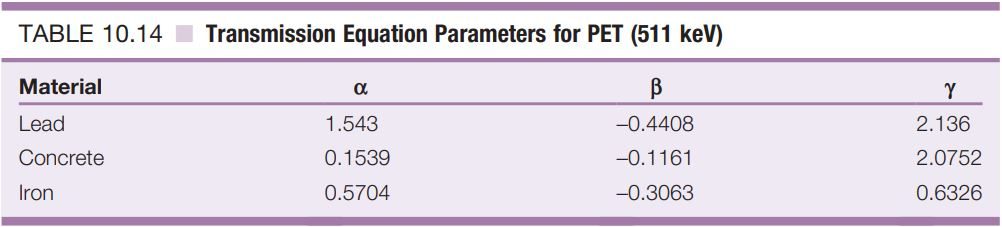
\includegraphics[width=0.8\textwidth]{Imagens/prTransPet.JPG}
		}%
		\caption{Parâmetros de Equação de Transmissão PET (511 keV).}
		\label{fig:prTransPet}
	\end{figure}

	A blindagem para o componente de TC geralmente é menor do que para o componente de PET, mas deve ser avaliada para confirmar que não é necessária nenhuma blindagem adicional. O produto de dose por comprimento (DLP) será significativamente maior do que em uma TC convencional, uma vez que o comprimento da varredura é muito maior (1.25 a 1.5 m).

	

\subsection*{Blindagem LDR}
	
	Embora seja atualmente incomum, ainda existem instalações que utilizam o ${}^{137}\text{Cs}$ ou o ${}^{192}\text{Ir}$ para implantes de baixa taxa de dose (LDR) ao longo de 1 a 2 dias. O Relatório 47 da Agência Internacional de Energia Atômica (AIEA) descreve a metodologia de blindagem recomendada para essas instalações.

	A equação para calcular a atenuação de blindagem necessária ($B$) é a seguinte:

	\begin{equation}
		B = \frac{{P \times 1000 \times d^2}}{{S_k \times t \times n \times T}}
	\end{equation}

	\begin{exemplo}[Onde:]
		\begin{itemize}
			\item $\textcolor{DarkTurquoise}{P}$ é o objetivo de projeto em mSv/semana,
			\item $\textcolor{DarkTurquoise}{d}$ é a distância em metros,
			\item $\textcolor{DarkTurquoise}{S_k}$ é a força de kerma no ar em $\mu$Gy m²/h ou U,
			\item $\textcolor{DarkTurquoise}{t}$ é o tempo médio de um implante em horas,
			\item $\textcolor{DarkTurquoise}{n}$ é o número de implantes por semana,
			\item $\textcolor{DarkTurquoise}{T}$ é o fator de ocupação.
		\end{itemize}
	\end{exemplo}

	É importante ressaltar que 1000 $\mu$Sv é equivalente a 1 mSv e, para fótons, 1 Gy é equivalente a 1 Sv.

		\begin{figure}[!h]
			\centering
			\fcolorbox{DarkTurquoise}{white}{%
				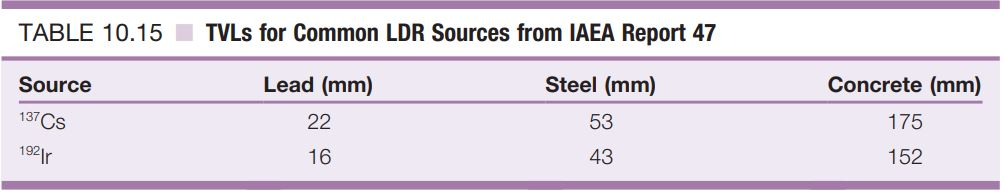
\includegraphics[width=0.8\textwidth]{Imagens/prTvlLDr.JPG}
			}%
			\caption{TVLs para Fontes LDR Comuns do Relatório 47 da AIEA.}
			\label{fig:prTransLDR}
		\end{figure}

	\begin{tcolorbox}[width=\textwidth, colback={white}, colbacktitle={DarkTurquoise!50!white}, title={$\bigstar$ \LobsterTwo{Exemplo: Blindagem LDR} $\bigstar $}, coltitle={CarnationPink}, colframe={DarkTurquoise}, fonttitle=\rmfamily\bfseries\Large]
		\begin{itemize}
			\item Para cada implante realizado, utiliza-se uma atividade de \SI{500}{U}, que é medida em força de kerma no ar. Além disso, temos uma média de tempo de \SI{50}{horas} por implante e realizamos dois implantes por semana. Ao inserir esses valores na equação de atenuação necessária, obtemos um valor de $B$ igual a \num{0.0036}. Esse valor representa a quantidade de atenuação requerida para alcançar a proteção adequada.

			\item A fim de calcular a espessura necessária para a blindagem, podemos utilizar o conceito de camadas decimais de valor (TVL). O TVL é determinado pelo logaritmo negativo de $B$ na base 10, ou seja, $\text{TVL} = -\log_{10}(B)$. No caso específico mencionado, encontramos um valor de TVL igual a \num{2.44}.
	
			\item A \ref{fig:prTransLDR}contém os valores de TVL para diversos materiais quando se trata de implantes utilizando o \ce{^{192}Ir} e o \ce{^{137}Cs}. Fazendo uso dos valores específicos para o chumbo, verificamos que seria necessário uma espessura de \SI{54}{mm} para o \ce{^{137}Cs} e \SI{39}{mm} para o \ce{^{192}Ir}, a fim de alcançar a blindagem desejada. Essa espessura é determinada para garantir a proteção adequada contra a radiação gerada durante os procedimentos de implante.
		\end{itemize}
	\end{tcolorbox}

	Na prática, realizar a blindagem completa de um quarto de paciente com chumbo para os implantes de baixa taxa de dose (LDR) seria uma opção custosa. Por esse motivo, geralmente são utilizadas proteções portáteis posicionadas próximas ao paciente, evitando a necessidade de blindar todo o ambiente. Essas proteções portáteis são projetadas de forma a garantir que a radiação seja adequadamente contida e não cause exposição desnecessária a outras áreas do ambiente.

	Uma estratégia recomendada é situar os quartos destinados aos implantes de LDR próximos a corredores ou banheiros, aproveitando o fato de que essas áreas tendem a ter menor ocupação. Dessa forma, é possível minimizar a exposição à radiação em áreas de maior tráfego, tornando o ambiente mais seguro tanto para os pacientes quanto para os profissionais envolvidos.

	Além disso, é importante considerar a duração dos implantes de LDR e o fator de uso associado a esses procedimentos. A taxa de dose instantânea (TDI), que se refere à taxa na qual a radiação é entregue em um determinado momento, deve ser limitada. Conforme sugerido pelo Relatório 47 da Agência Internacional de Energia Atômica (IAEA), para áreas não controladas, a TDI recomendada é de \SI{2.5}{\mu Sv/h} (0.25 mR/h). Já para áreas controladas, a TDI deve ser limitada a \SI{7.5}{\mu Sv/h} (0.75 mR/h). Esses valores visam garantir a segurança radiológica durante os procedimentos de implante e minimizar a exposição a radiações indesejadas para pacientes e profissionais envolvidos.


\subsection*{Blindagem HDR}

	Para fontes de alta taxa de dose (HDR), o cálculo da blindagem segue uma abordagem semelhante ao das fontes de baixa taxa de dose (LDR). As fontes HDR geralmente possuem uma força inicial de kerma no ar de 41.000 U e tempos de tratamento da ordem de 15 minutos. Supondo que sejam realizados 20 tratamentos por semana, podemos calcular a espessura de blindagem necessária para uma área não controlada a uma distância de 3 metros, considerando um fator de ocupação de 1.

	Com base nos dados fornecidos, a espessura de blindagem necessária seria de aproximadamente 49 mm de chumbo para garantir a proteção adequada na área não controlada. Essa espessura é calculada levando em consideração a taxa de dose produzida pela fonte HDR, a distância de 3 metros e o fator de ocupação. O objetivo é limitar a exposição à radiação em níveis seguros para as pessoas presentes na área não controlada.

	Da mesma forma, para uma área controlada situada a uma distância de 3 metros da fonte HDR, com um fator de ocupação de 1, seria necessária uma espessura de blindagem de aproximadamente 38 mm de chumbo. Essa espessura é determinada usando os mesmos princípios de cálculo mencionados anteriormente, visando garantir a segurança radiológica e minimizar a exposição a radiações indesejadas nas áreas controladas.

	É importante ressaltar que esses valores de espessura de blindagem são apenas estimativas com base nos parâmetros fornecidos. Para projetos reais, é essencial realizar cálculos mais detalhados considerando as características específicas do HDR utilizado, as taxas de dose esperadas e as normas de segurança aplicáveis. A orientação de documentos normativos, como o Relatório 47 da IAEA, fornece diretrizes adicionais para a seleção e implementação adequada da blindagem em instalações que utilizam fontes HDR.

\subsection*{Blindagem Prótons}

	O Particle Therapy Cooperative Group (PTCOG) publicou um relatório abordando a questão da blindagem para aceleradores de partículas, o qual pode ser encontrado em seu site oficial no endereço \href{http://www.ptcog.ch/index.php/ptcog-publications}{http://www.ptcog.ch/index.php/ptcog-publications}. É importante destacar que o projeto e a instalação da blindagem para aceleradores de partículas são geralmente realizados por equipes especializadas, que possuem conhecimentos técnicos e experiência nessa área. Portanto, embora físicos médicos gerais possam não estar diretamente envolvidos no processo de projeto da blindagem, eles devem ter conhecimento sobre as considerações e requisitos relacionados.

	No contexto dos aceleradores de partículas, é essencial abordar a questão da radiação secundária gerada durante diversas etapas de operação, como injeção, aceleração, extração, degradação de energia e transporte de partículas ao longo da linha de feixe. Além disso, a radiação secundária também pode ser gerada dentro do paciente ou do dispositivo de parada do feixe. Diante disso, é necessário aplicar a blindagem adequada em toda a instalação que abriga o acelerador, visando proteger as pessoas e minimizar a exposição a essa radiação.

	No cálculo da blindagem para aceleradores de partículas, os nêutrons desempenham um papel fundamental. Ao contrário dos fótons, a produção de nêutrons em aceleradores de partículas é predominantemente direcionada para a frente, em vez de ser isotrópica. Dessa forma, ciclotrons, que utilizam um degradador de feixe para obter energias mais baixas, requerem uma blindagem mais robusta em comparação com sincrotrons. Além disso, feixes de espalhamento passivo exigem uma blindagem mais eficiente do que feixes de varredura por raios estreitos, devido à produção de radiação secundária durante o processo de dispersão.

	No que diz respeito à escolha dos materiais de blindagem para aceleradores de partículas, é importante considerar que nêutrons de alta energia são mais efetivamente atenuados pelo uso de aço, em vez de concreto. No entanto, é essencial revestir a blindagem de aço com um material rico em hidrogênio, que tem a propriedade de absorver nêutrons de energia mais baixa. O relatório publicado pelo PTCOG fornece exemplos de espessuras de blindagem recomendadas para diferentes instalações, onde as espessuras de concreto variam de 1,2 a 4 metros, dependendo das características específicas do acelerador de partículas.

	Um aspecto crítico a ser considerado em instalações de partículas é a ativação dos materiais que se encontram na trajetória do feixe, especialmente em relação às aberturas do feixe e aos compensadores de alcance, que são manuseados pela equipe. Essa ativação deve ser cuidadosamente avaliada, levando em conta a segurança do pessoal envolvido no manuseio desses materiais e minimizando os riscos de exposição à radiação.

	Em resumo, a blindagem para aceleradores de partículas é uma área especializada que requer expertise específica no projeto e na implementação de soluções de proteção radiológica adequadas. O relatório do PTCOG é uma valiosa fonte de referência para orientar as práticas de blindagem nessas instalações, oferecendo diretrizes e exemplos práticos que contribuem para a segurança dos profissionais e dos pacientes envolvidos na terapia com partículas.

\subsection*{Avaliação das Blindagens}

	De acordo com o NCRP-151 (Conselho Nacional de Proteção contra Radiação e Medidas), é recomendado realizar uma avaliação abrangente da blindagem em cada nova instalação ou sempre que houver alterações nos pressupostos de um cálculo de blindagem existente. Para garantir uma avaliação completa, o relatório de avaliação deve conter os seguintes componentes:

	\begin{enumerate}[label=\textcolor{CarnationPink}{(\roman*)}]
		\item \textcolor{DarkTurquoise}{\textbf{Página de título}}: Essa página deve fornecer informações importantes, como a fonte de radiação, o nome da instalação e detalhes sobre as pessoas responsáveis pelos cálculos e medições, bem como aquelas que prepararam o relatório.

		\item \textcolor{DarkTurquoise}{\textbf{Revisão dos cálculos}}: Nessa seção, deve ser fornecida uma descrição detalhada dos cálculos utilizados para determinar os requisitos de blindagem. Isso inclui uma visão geral da metodologia adotada, das equações utilizadas e dos pressupostos aplicados na análise de blindagem.

		\item \textcolor{DarkTurquoise}{\textbf{Inspeção da construção}}: É importante descrever a inspeção realizada durante a fase de construção da instalação. Isso envolve a verificação de que os materiais de blindagem estão instalados corretamente e de acordo com as especificações de projeto.

		\item \textcolor{DarkTurquoise}{\textbf{Métodos de medição}}: Os detalhes sobre os métodos de medição empregados devem ser fornecidos. Isso inclui informações sobre as técnicas de medição utilizadas, a instrumentação empregada, os parâmetros de operação da máquina durante as medições e a metodologia utilizada para calcular o equivalente de dose (H) a partir dos dados obtidos nas medições.

		\item \textcolor{DarkTurquoise}{\textbf{Plantas baixas}}: A inclusão de plantas baixas é fundamental para compreender a distribuição espacial dos níveis de radiação dentro da instalação. Essas plantas devem indicar os locais onde as medições foram realizadas, proporcionando uma visão mais clara da distribuição de radiação ao redor do bunker.

		\item \textcolor{DarkTurquoise}{\textbf{Instrumentação}}: É importante fornecer informações detalhadas sobre os instrumentos utilizados para as medições, incluindo números de série e certificados de calibração. Isso garante a rastreabilidade e a precisão dos dados obtidos durante as medições.

		\item \textcolor{DarkTurquoise}{\textbf{Resultados das medições}}: Os resultados das medições realizadas em vários locais ao redor do bunker devem ser apresentados. Isso inclui informações como o equivalente de dose (H), a taxa média de dose-equivalente no tempo (TADR), a taxa de dose instantânea (IDR) e a dose máxima em qualquer momento.

		\item \textcolor{DarkTurquoise}{\textbf{Conclusões e recomendações}}: Essa seção deve resumir as principais conclusões da avaliação de blindagem e fornecer recomendações com base nos resultados obtidos. Isso pode incluir sugestões de melhorias ou modificações no projeto de blindagem, caso sejam necessárias.

		\item \textcolor{DarkTurquoise}{\textbf{Cópia do relatório}}: É fundamental manter uma cópia do relatório de avaliação de blindagem na própria instalação. Essa cópia servirá como referência e estará disponível para fins de conformidade regulatória.

		\item \textcolor{DarkTurquoise}{\textbf{Pesquisa de acompanhamento}}: Caso sejam necessárias modificações ou ajustes na blindagem da instalação, é recomendado realizar uma pesquisa de acompanhamento para verificar a eficácia das alterações feitas.
	\end{enumerate}

	A inclusão desses componentes no relatório de avaliação de blindagem garante que todo o processo seja documentado de forma completa, fornecendo uma compreensão abrangente das capacidades de blindagem contra radiação da instalação e auxiliando no monitoramento e na manutenção da segurança radiológica.

\subsection*{Monitoramento de Proteção Radiológica}

	Após a operacionalidade do acelerador linear (linac) e a produção de radiação, é essencial realizar uma pesquisa em todas as áreas ocupadas para garantir que os níveis de radiação estejam dentro dos limites permitidos. Esse processo de pesquisa envolve as seguintes etapas:

	\begin{enumerate}[label=\textcolor{CarnationPink}{\arabic*${}^\circ$}]
		\item \textcolor{DarkTurquoise}{\textbf{Uso de um detector GM ou instrumento similar:}} Um detector Geiger-Müller (GM) ou outro instrumento com capacidade de resposta rápida é utilizado para identificar defeitos na blindagem e identificar áreas com possíveis taxas de dose elevadas. Essa etapa permite uma inspeção preliminar das áreas ocupadas em busca de possíveis problemas de radiação.

		\item \textcolor{DarkTurquoise}{\textbf{Medição da taxa de dose máxima:}} Uma vez identificada a área com a maior taxa de dose preliminarmente, é realizada uma medição mais precisa da taxa de dose utilizando uma câmara de ionização calibrada ou um instrumento com mínima dependência energética. Essa medição é realizada a uma distância padronizada de 30 cm da parede para documentar os níveis de radiação nessa área específica.

		\item \textcolor{DarkTurquoise}{\textbf{Medição de nêutrons:}} Para instalações que utilizam feixes de energia acima de 10 MV, é necessário utilizar um medidor de nêutrons para medir os níveis de radiação de nêutrons. Essas medições de nêutrons são importantes devido aos requisitos específicos de blindagem para esse tipo de radiação e ao impacto potencial na segurança radiológica.
	\end{enumerate}

	É importante ressaltar que a área imediatamente adjacente ao bunker nem sempre é o fator limitante para a barreira de blindagem, uma vez que variações nos fatores de ocupação e fatores como o "skyshine" (radiação refletida no céu) também precisam ser considerados na avaliação dos níveis de radiação.

	Considerando as barreiras primárias e secundárias, existem algumas considerações específicas:

	\begin{itemize}[label=\textcolor{CarnationPink}{\textbullet}]
		\item \textcolor{DarkTurquoise}{\textbf{Barreiras primárias:}} As medições para barreiras primárias devem ser realizadas com o tamanho máximo do campo de radiação e sem a presença de um fantoma (simulador de tecido humano). Atenção especial deve ser dada aos ângulos de gantry que incidem nos cantos do chão e teto, pois a radiação refletida no céu e no solo pode contribuir para taxas de dose mais altas nessas regiões. As medições são normalmente feitas a uma distância padronizada de 30 cm da parede ou do chão.

		\item \textcolor{DarkTurquoise}{\textbf{Barreiras secundárias:}} As medições para barreiras secundárias são realizadas com o tamanho máximo do campo de radiação e um fantoma colocado no feixe. Essas medições são importantes para avaliar a eficácia da blindagem em áreas onde o feixe interage com componentes secundários, como colimadores e acessórios de tratamento.
	\end{itemize}

	Nos casos em que o linac está localizado em uma estrutura de prédio sem áreas ocupadas acima dele, também é necessário realizar pesquisas no telhado para garantir a segurança radiológica e o cumprimento dos requisitos de blindagem. Essas medidas adicionais são importantes para garantir que a radiação seja adequadamente controlada em todas as áreas relacionadas ao linac.


\subsection*{Gerenciamento de Fontes Radioativas}

	Ao receber fontes radioativas em um departamento, é essencial seguir procedimentos específicos para garantir a segurança e responsabilidade adequadas. Embora as regulamentações possam variar de acordo com a jurisdição, existem algumas características comuns que devem ser consideradas. Os principais pontos a serem observados são:

	\begin{enumerate}[label=\textcolor{CarnationPink}{\arabic*.}]
		\item \textcolor{DarkTurquoise}{\textbf{Inspeção da embalagem:}} A embalagem recebida deve ser prontamente inspecionada, dentro de um prazo de até 3 horas, para determinar se os níveis de exposição estão dentro dos limites aceitáveis. Isso é geralmente feito usando instrumentos de detecção de radiação adequados para verificar a radiação emitida pela fonte.
		
		\item \textcolor{DarkTurquoise}{\textbf{Categorização dos envios:}} O Departamento de Transporte dos Estados Unidos (DOT) categoriza os envios de fontes radioativas com base em leituras de exposição na superfície da embalagem e a uma distância de 1 metro. Existem três categorias: Amarela II, Amarela III e categorias mais altas (\ref{fig:prEmbalados}). Essa categorização é importante para determinar as precauções e requisitos de segurança apropriados para o manuseio e transporte dessas fontes.
		
		\item \textcolor{DarkTurquoise}{\textbf{Índice de transporte (TI):}} Embalagens classificadas como Amarela II e Amarela III requerem um índice de transporte (TI). O TI é calculado arredondando a leitura de exposição a 1 metro em mR/h (milirrem por hora) para a décima mais próxima, sem unidades. Por exemplo, se a leitura for 0,26 mR/h, o TI seria 0,3. O TI é usado para fins de identificação e controle adequado durante o transporte.
		
		\item \textcolor{DarkTurquoise}{\textbf{Verificação de contaminação superficial:}} É essencial verificar a superfície da embalagem quanto à contaminação removível. Isso é feito realizando um teste de limpeza em uma área específica da embalagem (por exemplo, 300 cm\textsuperscript{2}) e medindo a atividade (em desintegrações por minuto, dpm) no material coletado. Limites regulatórios, como o limite de 6600 dpm/300 cm\textsuperscript{2} estabelecido pela Comissão Reguladora Nuclear dos Estados Unidos (NRC) no 10 CFR 20, devem ser seguidos para garantir que a contaminação esteja dentro de limites aceitáveis.
		
		\item \textcolor{DarkTurquoise}{\textbf{Manuseio seguro e controle de inventário:}} Materiais radioativos devem ser armazenados e manuseados com segurança em todos os momentos para garantir um controle adequado do inventário. Isso inclui medidas para evitar perdas, roubos ou acesso não autorizado aos materiais. As práticas de armazenamento e manuseio devem seguir as diretrizes e procedimentos estabelecidos pelas regulamentações aplicáveis.
		
		\item \textcolor{DarkTurquoise}{\textbf{Registro de informações:}} É essencial manter um registro detalhado para registrar o recebimento, uso e descarte de todas as fontes radioativas. Esse registro permite um rastreamento adequado e a responsabilidade das fontes radioativas, além de facilitar a conformidade com as regulamentações e diretrizes aplicáveis.
	\end{enumerate}

	Ao aderir a esses procedimentos, é possível garantir um manuseio seguro, transporte adequado e controle efetivo das fontes radioativas, em conformidade com as regulamentações e diretrizes específicas da área. Essas medidas são essenciais para proteger a saúde e segurança dos profissionais envolvidos, bem como do público em geral.

		\begin{figure}[!h]
			\centering
			\fcolorbox{DarkTurquoise}{white}{%
				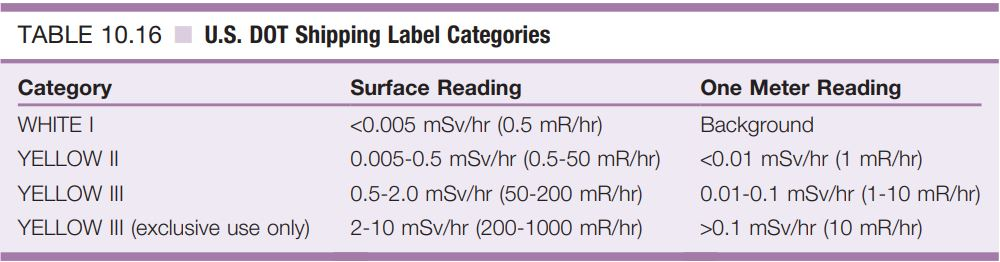
\includegraphics[width=0.8\textwidth]{Imagens/prEmbalados.JPG}
			}%
			\caption{Categorias de etiquetas de remessa DOT dos EUA.}
			\label{fig:prEmbalados}
		\end{figure}

\subsection*{Treinamento de Proteção Radiológica}

	NCRP-134 identifica quatro motivos para fornecer treinamento em segurança radiológica:

	\begin{enumerate}
			\item \textcolor{DarkTurquoise}{\textbf{Desenvolvimento de habilidades:}} O treinamento permite que a equipe execute tarefas com mais eficiência e confiança, adquirindo o conhecimento e as habilidades necessárias.
			
			\item \textcolor{DarkTurquoise}{\textbf{Conscientização e redução de riscos:}} O treinamento aumenta a conscientização sobre os riscos associados à exposição à radiação, incentivando as pessoas a participarem ativamente na aceitação e redução desses riscos sempre que possível.
			
			\item \textcolor{DarkTurquoise}{\textbf{Redução de acidentes:}} O treinamento adequado ajuda a diminuir o número e a gravidade de acidentes relacionados à radiação, promovendo práticas seguras e adesão a protocolos.
			
			\item \textcolor{DarkTurquoise}{\textbf{Conformidade regulatória:}} Funcionários devidamente treinados se tornam cientes dos requisitos regulatórios e podem garantir a conformidade com as regulamentações de segurança radiológica.
		\end{enumerate}

	Para identificar os requisitos de treinamento, vários fatores devem ser considerados, incluindo:

	\begin{itemize}
		\item \textcolor{DarkTurquoise}{\textbf{Potencial de exposição:}} O nível potencial de exposição à radiação nas tarefas realizadas pela equipe.
		
		\item \textcolor{DarkTurquoise}{\textbf{Complexidade das tarefas:}} A complexidade das tarefas envolvendo radiação, que pode exigir habilidades e conhecimentos específicos.
		
		\item \textcolor{DarkTurquoise}{\textbf{Requisitos regulatórios:}} Conformidade com regulamentações e diretrizes de segurança radiológica.
		
		\item \textcolor{DarkTurquoise}{\textbf{Nível de conhecimento em física:}} O nível de compreensão da física da radiação necessário para as tarefas.
		
		\item \textcolor{DarkTurquoise}{\textbf{Nível de supervisão:}} O nível de supervisão da equipe, pois funcionários com menos supervisão podem exigir treinamento mais abrangente.
		
		\item \textcolor{DarkTurquoise}{\textbf{Funções de supervisão:}} Treinamento adicional pode ser necessário para indivíduos em cargos de supervisão.
		
		\item \textcolor{DarkTurquoise}{\textbf{Treinamento anterior:}} Qualquer treinamento prévio em segurança radiológica que a equipe tenha recebido.
		
		\item \textcolor{DarkTurquoise}{\textbf{Preocupações da equipe:}} Abordar preocupações ou perguntas específicas levantadas pela equipe em relação à segurança radiológica.
	\end{itemize}

O desenvolvimento de um programa de treinamento geralmente envolve seis etapas:

	\begin{enumerate}
		\item \textcolor{DarkTurquoise}{\textbf{Análise das tarefas do trabalho:}} Analisar as competências necessárias para executar com segurança as tarefas relacionadas à radiação.
		
		\item \textcolor{DarkTurquoise}{\textbf{Design e desenvolvimento do treinamento:}} Determinar a natureza do perigo da radiação, tamanho do grupo, habilidades, conhecimentos, atitudes necessárias, recursos disponíveis, objetivos do treinamento, critérios de avaliação e estrutura do curso.
		
		\item \textcolor{DarkTurquoise}{\textbf{Esboço do curso e materiais de treinamento:}} Desenvolver o esboço detalhado e os materiais de treinamento necessários.
		
		\item \textcolor{DarkTurquoise}{\textbf{Plano de avaliação:}} Estabelecer um plano para avaliar a eficácia do treinamento, incluindo avaliação de reação, avaliação de aprendizado, avaliação de desempenho e avaliação de resultados.
		
		\item \textcolor{DarkTurquoise}{\textbf{Instrução de treinamento:}} Fornecer o treinamento real para a equipe, que pode ser ministrado em vários formatos, como estudo individual, instrução em grupo, mentoria ou treinamento no local de trabalho.
		
		\item \textcolor{DarkTurquoise}{\textbf{Avaliação e feedback:}} Seguir o plano de avaliação e coletar feedback para avaliar a eficácia do programa de treinamento e dos instrutores.
	\end{enumerate}

É importante auditar periodicamente o programa de treinamento para garantir um registro adequado, avaliar a eficácia do programa e avaliar o desempenho dos instrutores.

O NCRP fornece uma lista sugerida de tópicos para treinamento em segurança radiológica, que pode servir como um guia para o desenvolvimento do programa de treinamento.

\end{document}

		\begin{figure}[!h]
			\centering
			\fcolorbox{DarkTurquoise}{white}{%
				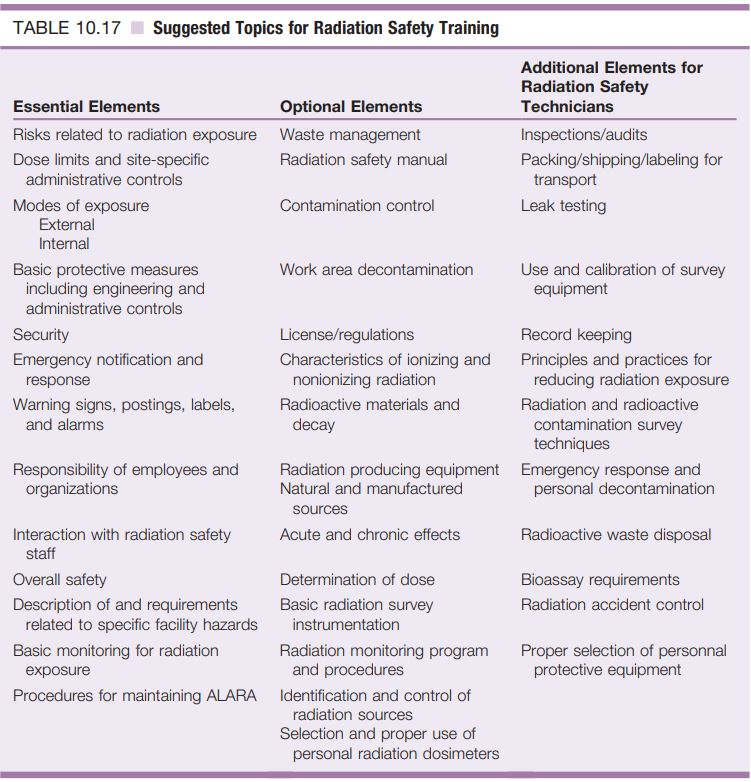
\includegraphics[width=0.8\textwidth]{Imagens/prTreinamento.JPG}
			}%
			\caption{Tópicos sugeridos para treinamento de proteção radiológica.}
			\label{fig:prTreinamento}
		\end{figure}


\bibliography{ref.bib}
\end{document}